%!TEX root = ../thesis.tex
\chapter{Introduction}

%!TEX root = ../thesis.tex
\section{Motivation}

In recent years the web has become a ubiquitous platform\footnote{More than 3/4 of the people in developed countries have access to the Internet both via a computer and via a mobile device. \cite{ITU2013}} which is used by many on a daily basis. Its usage has changed dramatically over time and has developed from primarily being a source of information to being a platform that is used for social activities, entertainment and productive work. This change has been driven by standardized technological innovation of the browsers vendors, which allow developers to build more complex and more interactive applications. In the last few years for example, APIs for advanced network access, APIs for peer-to-peer communication and APIs for 3D rendering have been standardized and been introduced in modern web browsers.

Modern web applications very often allow its users to collaborate and to interact with one another. Either by allowing social interactions like messaging other users or to comment on user-generated content or by allowing users to work together collaboratively like in Google Docs. Especially the case of Google Docs has shown how powerful collaborative work on the web can be. Collaborative web applications benefit from many years of research and experience in desktop-based synchronization algorithms and more and more applications are starting to introduce these algorithms.

A new addition to the list of novel APIs is the Web Audio API which gives access to advanced low-level audio features that can be used to precisely compose music and to produce sounds synthetically. Since the API had been introduced in the first browsers, a lot of interactive sound experiments had been created that showed what kind of applications are now possible to create by only using web technology. The API is still marked as being an early draft, but its web browser implementations are already stable enough to build applications on top of it.

The purpose of this thesis is to build a prototypical collaborative web-based Digital Audio Workstation (DAW) on top of the Web Audio API and on top of new communication APIs which serve as a synchronization channel. Digital Audio Workstations have existed for many years as desktop application and they allow users to create songs entirely digital. This thesis acts as a test to try out the limitations of the Web Audio API and the web as a platform for a replacement or as an addition to existing DAW applications. Furthermore, it is a test to see how good collaboration works in DAWs, because most DAWs do not feature collaborative editing.

\section{Disclaimer}

At the time the work on this thesis started, the above mentioned approach was a complete novelty. But during the development phase the software `Soundtrap'\footnote{\url{https://www.soundtrap.com/}, accessed at 28.03.2014} by `Playwerk AB' has been released in an early alpha stage. It is a similar product to the application that will be described in this thesis. Soundtrap, however, is based on a completely different technology stack and algorithms. Additionally, it is not sure if the collaborative feature of that editor uses one of the enhanced synchronization algorithms described here.

\section{Structure}

The first part of this thesis (\refchapter{part:theory}) contains the theoretical background that is needed in order to implement collaborative audio editing software. \refchapter{ch:audio-theory} dives into the backgrounds of digital signal processing and how it can be realized in modern web applications. \refchapter{ch:sync-theory} then shows different concepts of data synchronization and discusses which approach is most suitable for the application of this thesis. \refchapter{ch:realtime-theory} lists and describes the available communication technologies on the web and examines, which of the presented technologies is most suitable for the chosen synchronization model.

The second part (\refchapter{part-concept}) explains the concept of the application. In \refchapter{ch:concept-editor} all the editor's components are listed. Furthermore, it is explained why exactly these components were chosen and how they compare to the components in other DAWs.

The third part (\refchapter{part:implementation}) is about how the application that was described in \refchapter{part-concept} has been implemented. \refchapter{ch:impl-editor} goes into the implementation details and techniques of each of the editor's components. The web application that was built around it is explained in \refchapter{ch:impl-backend}. The implementation of the synchronization algorithm and the enhancements that were made during this thesis are explained in \refchapter{impl-sync-algorithm}.

The fourth and last part of thesis (\refchapter{part:conclusion}) then evaluates (\refchapter{ch:evaluation}) the application prototype and the state of audio processing on the web and gives a future outlook on further improvements and additions that will be made to the editor (\refchapter{ch:outlook}).

\part{Theory}
\label{part:theory}

\chapter{Audio and the Web Audio API}
\label{ch:audio-theory}

%!TEX root = ../../thesis.tex

\section{Evolution of Audio on the Web}
\label{sec:webaudio-evolution}

\begin{quote}
  ``So if you really want advanced features, I recommend embedding MP3 files via a Flash-based player instead.'' - \url{http://www.boutell.com/newfaq/creating/midi.html}
\end{quote}

In the history of HTML, audio never played a big part, naturally because HTML was intended for sharing scientific documents and not for the purpose that it has evolved into these days; to serve highly interactive and multimedia-capable applications. Despite this, there were several approaches to at least embed sound into HTML websites. Internet Explorer, for example, introduced a non-standard element called \code{bgsound}\footnote{\url{http://msdn.microsoft.com/en-us/library/ie/ms535198(v=vs.85).aspx} (10.02.2014)} which would load and play an audio file that was specified in the \code{src} attribute. It was also possible to specify the \code{volume}, the \code{balance}\footnote{Difference in volume between the left and the right speaker.} and if the sound should \code{loop}. Since the \code{bgsound}-element was not standardized, all other browsers simply ignored it and sound would only play in Internet Explorer. Also, it was not possible to control the element with JavaScript and the sound would only play until it was over (or it would play infinitely). Nowadays even Microsoft discourages the usage of this element: ``This element is obsolete and should no longer be used''. \cite{msdn2014bgsound}

Other proposals to play audio on the web were mostly based on using external plugins to play audio. The two important elements that played (or still play, as explained later) a role here were \code{object} and its successor \code{embed}. They were designed for embedding content into HTML that could not be displayed by other HTML elements, content like flash movies, videos, Java applets and audio files. When parsing such an element, the browser would look up and start one of its plugins to display the content. So if we wanted to embed an audio file for example, one of the user's media players would get injected into the page including its native media controls. Still, it was not possible to script the behavior of the element and sound files would not play if a user did not have a media player installed. \cite[The embed element]{w32014html5}

Adobe's Flash player became very popular amongst web developers because it provided all the needed APIs for adding and controlling multimedia objects and even games on web sites. So in order to play sounds on a website, developers simply included a flash script that would take some parameters (e.g. a song list) from the \code{embed} element and Flash would then take care of playing them. Some of these players had their own interface for playing and skipping songs from playlists (e.g. XSPF Web Music Player\footnote{\url{http://musicplayer.sourceforge.net/}}) and some only acted as scriptable player objects and developers were able to provide their own HTML interface and to control the playback with JavaScript. These players worked well in the cases that developers needed media player replacements on their websites, because Flash was, and still is, available on more than 95\% of all Internet-connected PCs. \cite{arah200999percent}

Nevertheless, using these players meant that developers were depending on Flash, a proprietary, licensed technology, to add multimedia capabilities to their websites, which is in stark contrast to the open nature of the web. Therefore, a new HTML element was introduced in HTML5; the \code{audio} element\footnote{\cite[The audio element]{w32014html5}}. This new element finally gives developers the opportunity to play audio files on their websites through a standardized and widely available\footnote{\url{http://caniuse.com/audio}, last checked on 24/03/2014} API.

\begin{lstlisting}[language=HTML, caption=The HTML5 audio element, label=lst:audioelement]
  <audio id="my_audio" controls preload autoplay>
    <source src="sound.mp3" type="audio/mpeg" />
    <source src="sound.ogg" type="audio/ogg" />
  </audio>
\end{lstlisting}

The element (see \reflisting{lst:audioelement}) consists of the enclosing \code{audio} tag and various \code{source} tags. Each \code{source} tag stands for a different file format of the same audio file so that browsers can decide which file to pick, depending on the codecs that are available. Developers can control the behavior of the \code{audio} tag by adding several attributes to it, like the \code{preload} attribute, which will ensure that the audio file is preloaded once the element has been rendered, or the \code{autoplay} attribute which will play the audio file automatically after enough data of the file has been buffered.

\begin{lstlisting}[language=JavaScript, caption=Interacting with the audio element in JavaScript, label=lst:audioelementjs]
  var audio = document.getElementById("my_audio");

  var playBt = document.getElementById("play-button");
  playBt.addEventListener("click", function(){
    audio.play();
  });

  var stopBt = document.getElementById("stop-button");
  stopBt.addEventListener("click", function(){
    audio.stop();
  });
\end{lstlisting}

Just as with different flash libraries for audio playback, the \code{audio} element provides two possible modes. The `visual' mode, which provides a minimal interface for controlling the audio playback, is activated by adding the \code{controls} attribute to the element. When the \code{controls} attribute is omitted, the element is not rendered visually but it will still provide playback capabilities via JavaScript and developers can build with a custom user interface. \reflisting{lst:audioelementjs} demonstrates how to interact with the \code{audio} element in JavaScript. It can be selected just like all other DOM nodes by using \code{document.getElementById} (line 1) and it has several methods like \code{play} (line 5) and \code{stop} (line 10) to control the audio playback\footnote{\cite[Media elements]{w32014html5}}.

In addition to the above mentioned methods and attributes, the element's API also provides methods to change the audio file, to reload the audio file or to use audio streams as their source. All in all, the audio element provides a complete API to play back audio files of any kind on a website.

Now that there was a way to play audio, the logical next step was to add APIs to analyze and create audio. In 2010 \cite{kirn2010soundsynth}, a team at Mozilla started working on an extension to the \code{audio} element's API, the Audio Data API, that added features such as frequency analysis and writing raw audio via JavaScript. Though the API was only available in Firefox, and has never been implemented in another web browser, it already showed at that time, that audio processing in JavaScript is a field that many people are interested in and there were many demos, showing the capabilities of this draft API like beat detection algorithms or filter functions \cite[chapter: Working Audio Data Demos]{humphrey2013audiodata}.

The `successor' of the Audio Data API is the Web Audio API \cite{wilson2014webaudiospec}, which was drafted by Chris Rogers in 2012. It describes a more low-level audio API which adds important features like exact audio timing, detailed audio analysis and DSP\footnote{Digital Signal Processing} to JavaScript. These features are the building blocks of all modern audio programs and they now allow the development of complex audio visualizations and audio software in the browser. As of today\footnote{\url{http://caniuse.com/audio-api}, last checked on 18/02/2014}, the Web Audio API is available in the recent versions of Chrome, Safari, Opera and Firefox, as well as in iOS Safari, Chrome for Android and Firefox for Android.

\begin{lstlisting}[language=JavaScript, caption=Simple node graph in the Web Audio API, label=lst:webaudio-simple]
  var context = new AudioContext();

  var osc = context.createOscillator();
  var filter = context.createBiquadFilter();

  osc.connect(filter);
  filter.connect(context.destination);
\end{lstlisting}

The Web Audio API is, like many other audio-related APIs, a node-graph based API \cite[chapter: 1.1]{smus2013webaudio}. All nodes are created from a \code{context} object (line 1), just like in the \code{canvas} API\footnote{\url{http://www.w3.org/wiki/HTML/Elements/canvas}, last checked on 24/02/2014} (see \reflisting{lst:webaudio-simple}). Nodes can be connected to other nodes which can then alter or analyze the signal and pass it to the next node. In order to play the sound on the user's speakers, a node needs to be connected to the \code{context's destination} (line 7). In this example, an oscillator is connected to a filter (line 6) which filters the signal's frequencies and then passes it to the \code{destination}. The next chapters will focus on important audio-theory aspects and how they can implemented or used in the Web Audio API.
%!TEX root = ../../thesis.tex
\section{Buffers}
\label{sec:webaudio-buffer}

\begin{quote}
  ``Arrange whatever pieces come your way.'' -
  Virginia Woolf
\end{quote}

The foundation of every music production software is the ability to play back audio files. It is needed in DJing software to mix songs together, or in composition software to create sample based arrangements of various kinds (e.g. in sequencers or drum machines).

Though playing back audio files was already possible with the \code{audio} element, the Web Audio API (WAA) provides a new way to load and play files in order to make them available in its node-based system. Since the WAA is more low-level than other audio APIs before, loading a file and playing a file involve more than just a simple \code{audio} element that takes care of everything. 

\begin{lstlisting}[language=JavaScript, caption=Fetching an audio file from the server, label=lst:xhr-audio]
  var xhr = new XMLHttpRequest();
  xhr.open("GET", "/the_file.mp3", true);
  xhr.responseType = "arraybuffer";
  xhr.onload = processFile
  xhr.send();
\end{lstlisting}

The first step is to load a remote file into the application with an XHR request (see \reflisting{lst:xhr-audio}). It is important to set the \code{responseType} to \code{arraybuffer} (line 3) so that it can be processed properly by the WAA in the \code{processFile} callback (line 4).

\begin{lstlisting}[language=JavaScript, caption=Decoding the audio file, label=lst:processFile]
  context.decodeAudioData(xhr.response, function(buffer) {
    songBuffer = buffer;
  }, function(e) {
    console.log("Something went wrong", e);
  });
\end{lstlisting}

After receiving the file, the request's \code{response} needs to be decoded from an \code{AudioContext} instance (line 1, \reflisting{lst:processFile}), which will return the decoded file as an instance of \code{AudioBuffer} (line 2) that is needed in order to play the file. The WAA hides the complexity of deciding which decoder to use depending on the current file's format. In case of the current client not supporting the file format, the decode step will fail and call the second callback (line 4). In order to prevent this from happening, it comes in handy to use the \code{audio} element's \code{canPlayType} (\cite[MIME types]{w32014html5}) method to determine if an alternative file format should be used.

\begin{lstlisting}[language=JavaScript, caption=Playing the \code{AudioBuffer}, label=lst:playbuffer]
  var source = context.createBufferSource();
  source.buffer = songBuffer;
  source.connect(context.destination);
  source.start(0);
\end{lstlisting}

The last step is to create a \code{BufferSourceNode} (line 1, \reflisting{lst:playbuffer}) which is capable of hooking into WAA's node graph (line 3) and \code{starting} the \code{AudioBuffer} (line 4). A \code{BufferSourceNode} can be stopped by calling its \code{stop} method but the instance cannot be reused again, once it has been stopped. Every time an \code{AudioBuffer} should be played, a new instance of \code{BufferSourceNode} needs to be created.
%!TEX root = ../../thesis.tex
\section{Oscillators}
\label{sec:webaudio-osc}

\begin{quote}
  ``It's basic elements, like love, dancing and sine waves.'' -
  Eero Johannes (We call it Skweee)
\end{quote}

Oscillators in physics, and generally in the analog world, are devices that generate and form electronic signals. When they are wired together with speakers and produce frequencies within the human range of hearing (20Hz to 20kHz), they can be used to create electronic sounds. Depending on the type of wave that is used as an initial signal and the signal's frequency, sounds are softer, harder, higher (high frequency) or lower (low frequency). Oscillators build the foundation of electronic music production and they are the building blocks for many instruments (e.g. synthesizers) and techniques (e.g. LFO).

\begin{figure}[htb]
  \centerline{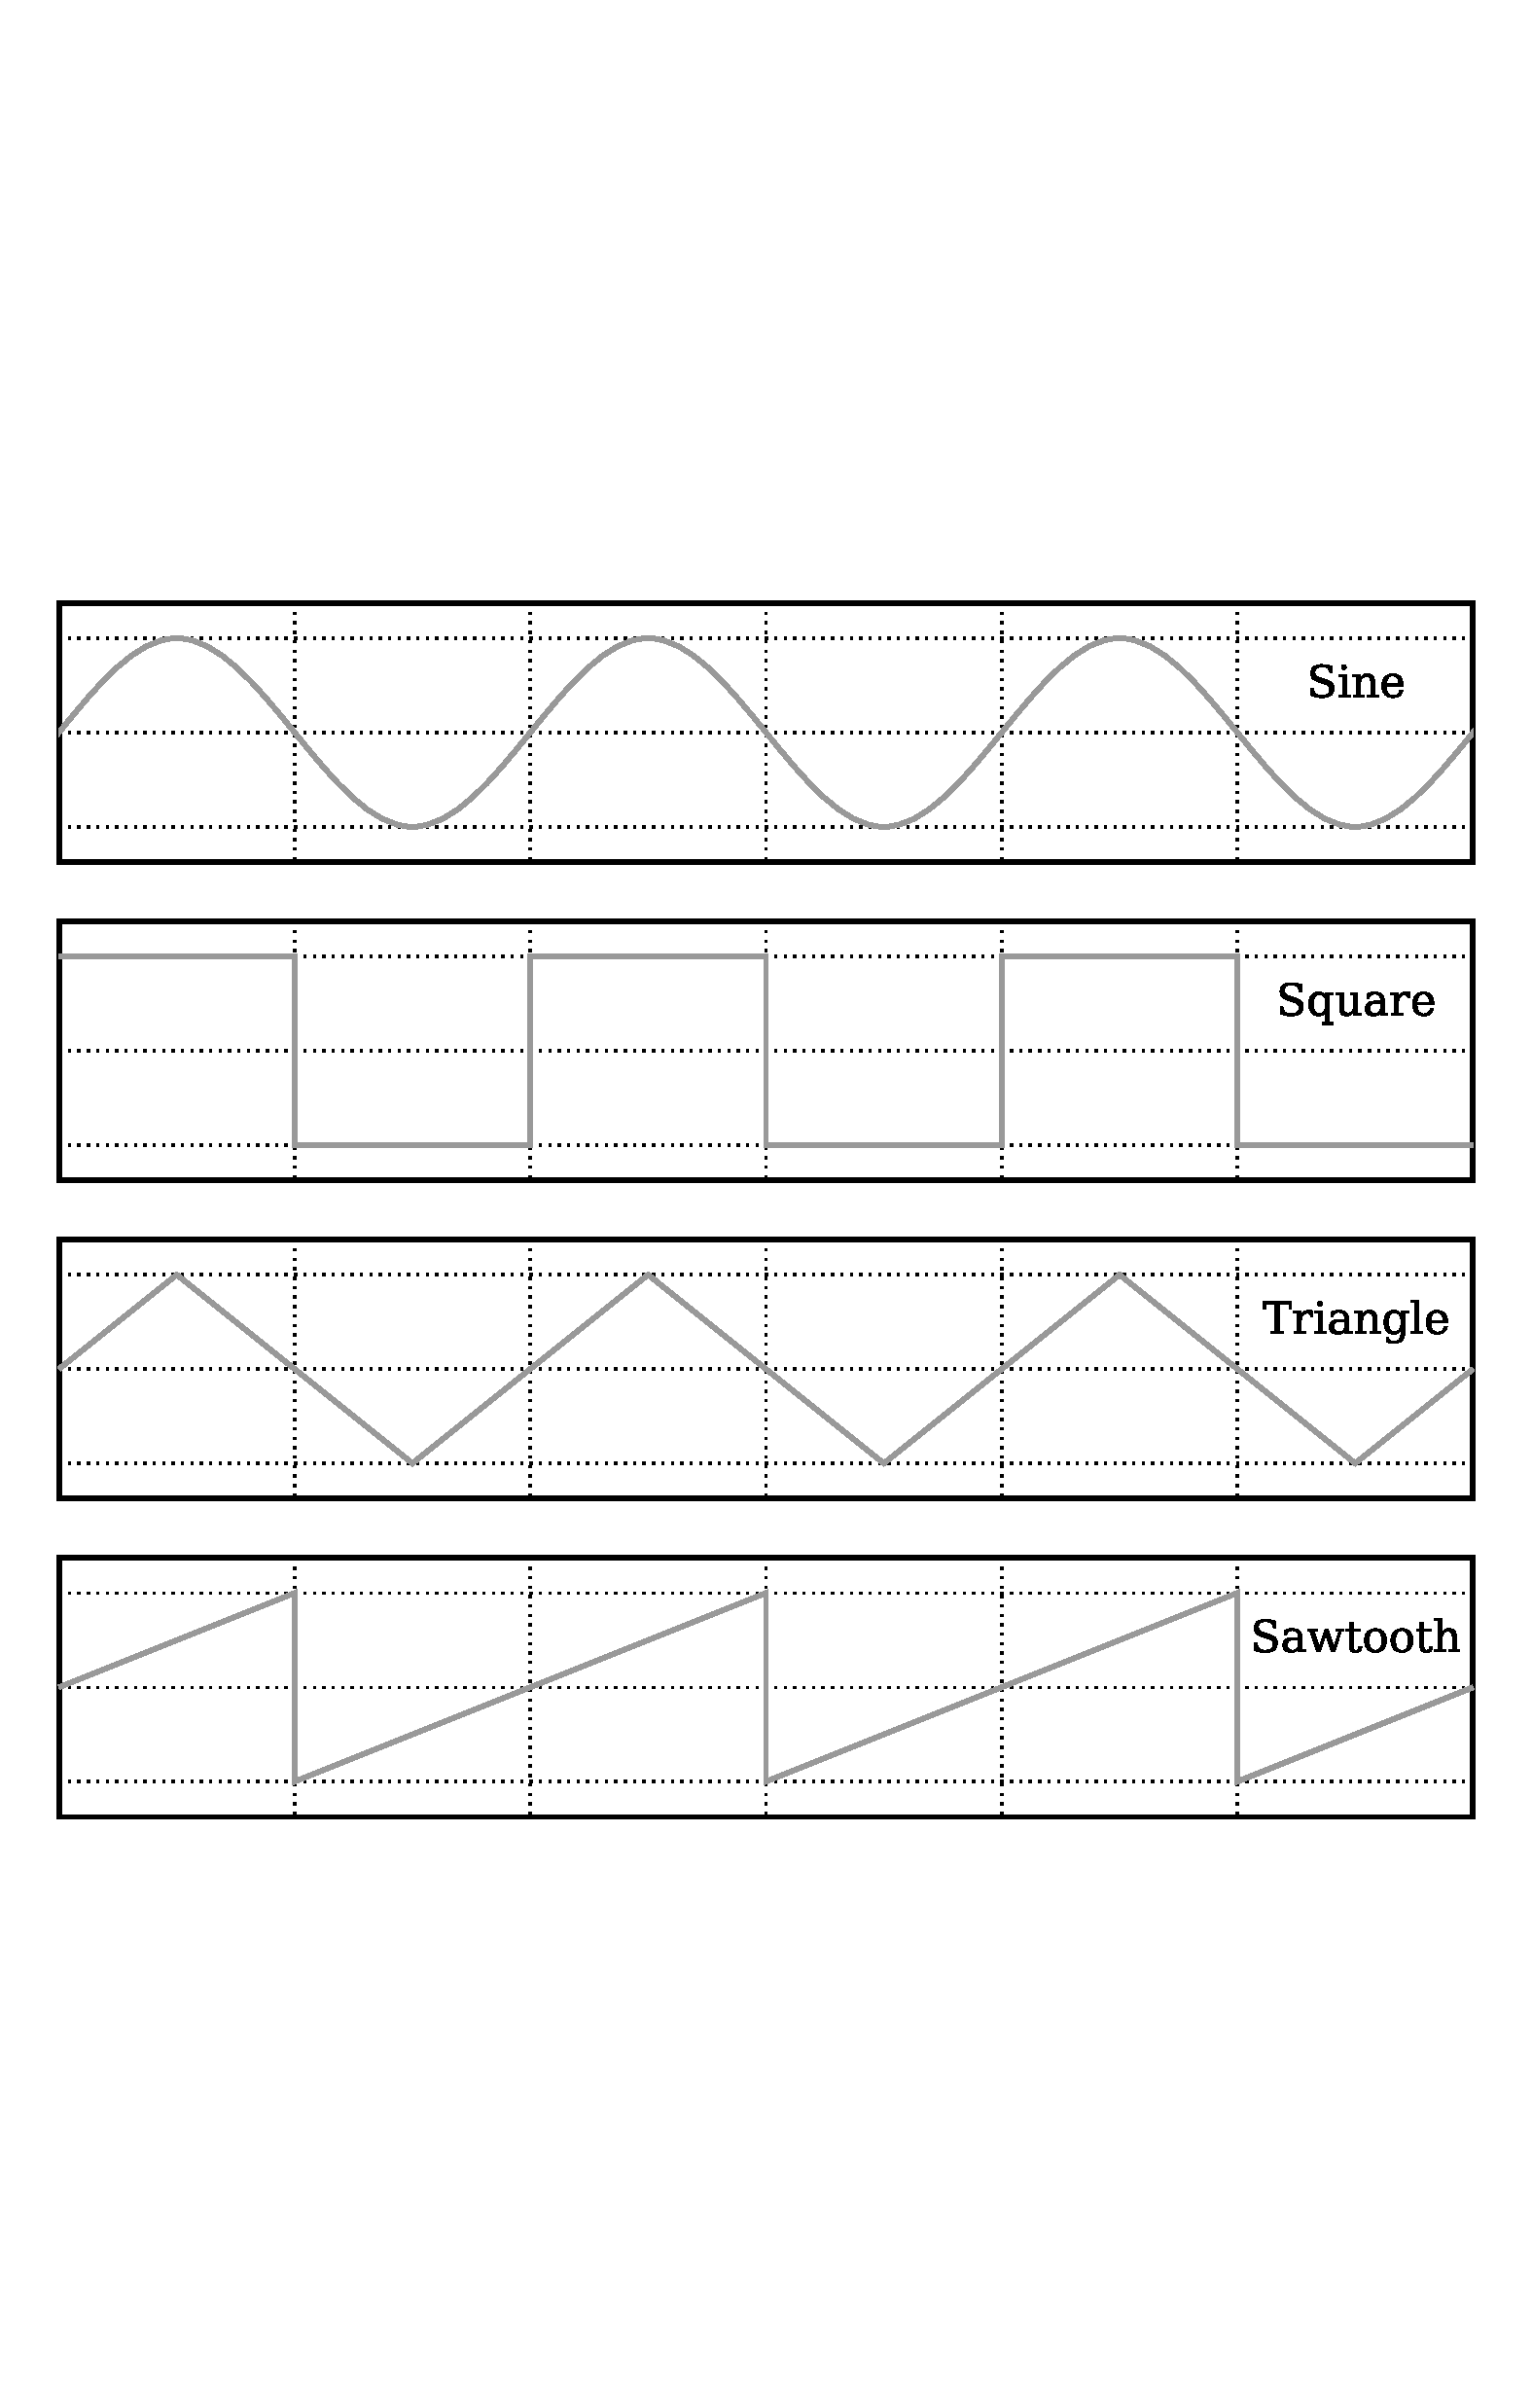
\includegraphics[width=0.8\linewidth]{images/Waveforms.pdf}}
  \caption[The different waveforms supported by the Web Audio API -
  \protect\newline{\small\url{http://en.wikipedia.org/wiki/File:Waveforms.svg} (20.02.2014)}
  \protect\newline{\small\emph{WikiMedia - User:Omegatron}}]{The different waveforms supported by the Web Audio API}
  \label{fig:waveforms}
\end{figure}

Oscillators in the Web Audio API support four different wave types which are shown in figure \reffigure{fig:waveforms} \cite{wilson2014webaudiospec}. The sine wave is the most classical wave that produces a pure note without overtones and is very uncommon to be used on its own in music programming but it is very often used to thicken the sound of other waves \cite[chapter: 2, Sine Wave]{cannAnalogSynthesis}. Square waves are often used for bass sounds and to create ``woody and reedy tones''\footnote{\cite[chapter: 2, Square Wave]{cannAnalogSynthesis}}. Triangle waves have a similar sound to sine waves but are more sharp. In early synthesizers, which were not capable of producing pure sine waves, triangle waves were used instead\footnote{\cite[chapter: 2, Triangle Wave]{cannAnalogSynthesis}}. Sawtooth waves have a bright sound and they are very commonly used for further sound shaping and filtering. Even after filtering, their unique sound will shine through the sculpted sound\footnote{\cite[chapter: 2, Sawtooth Wave]{cannAnalogSynthesis}}.

\begin{lstlisting}[language=JavaScript, caption=Playing a sound from an oscillator, label=lst:webaudiooscillator]
  var oscillator = context.createOscillator();
  // 0 -> sine; 1 -> square; 2 -> sawtooth; 3 -> triangle
  oscillator.type = 0;
  oscillator.frequency.value = 22000;
  oscillator.connect(context.destination);
  // start the oscillator
  oscillator.start(0);
\end{lstlisting}

As any other \code{AudioNode}, \code{Oscillators} are created from an \code{AudioContext} instance and they have to be wired into the node graph in order to create sounds (see \reflisting{lst:webaudiooscillator}). In addition to the above described waves (line 2f), an arbitrary wave can be created from a \code{Float32Array} and assigned to an oscillator object\footnote{\cite[createPeriodicWave]{wilson2014webaudiospec}}. In this way, developers could, e.g., add the missing pulse wave with a specific distribution of on- and off-time. A square wave is basically a pulse wave with a distribution of 50\%. The \code{frequency} property is of the special type \code{AudioParam} and needs to be set via the object's \code{value} property, instead of assigning it directly because \code{AudioParams} provide ways to exactly time parameter values (see \refchapter{sec:webaudio-timing}).

Line 4 is again a reminder that it is important to not keep the range of human hearing (20Hz to 20kHz) in mind. It creates a wave with a frequency of 22kHz which humans are not able to hear but the Web Audio API is still capable of creating these sounds. Frequencies that are lower than the `minimum' 20Hz come in handy when Low Frequency Oscillators (see \refchapter{sec:webaudio-synth}) are used to create new sounds, although their bare signal cannot be heard by humans.
%!TEX root = ../../thesis.tex
\section{Filters}
\label{sec:webaudio-filter}

\begin{quote}
  ``It's quite ironic: We got rid of our analog equipment, replaced it with digital, then spent the next couple of decades trying to get the digital to sound like the analog we got rid of.'' -
  David Williams
\end{quote}

Audio filters allow for the manipulation of the frequency spectrum of a sound in order to create a certain effect on the sound or to sculpt a certain note so that it creates a different atmosphere in combination with other sounds. Each filter has several parameters that influence the effect on the source sound.

\begin{figure}[htb]
  \centerline{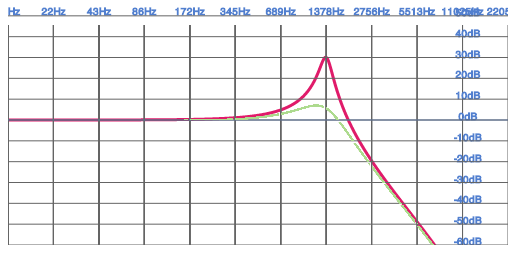
\includegraphics[width=0.9\linewidth]{images/filter-demonstration.png}}
  \caption[Visualization of a low-pass filter -
  \protect\newline{\small\url{http://webaudio-io2012.appspot.com/\#34} (01.03.2014)}
  \protect\newline{\small\emph{Chris Wilson}}]{Visualization of a low-pass filter (red: high Q, green: low Q)}
  \label{fig:filters-visualization}
\end{figure}

There is the \emph{cut-off} frequency parameter, which determines the level of frequency at which the filter should affect the sound. The example in \reffigure{fig:filters-visualization} shows a low-pass filter, which filters out lower frequencies. The cut-off frequency in this case is 1378Hz, the graph's peak, and the dB for higher frequencies is rapidly getting lower so they are not heard anymore. The next important parameter is the \emph{quality} factor of the filter which influences the steepness of the peak. The red line shows a filter with a higher \emph{quality} parameter than the green one. A low \emph{cut-off} frequency leads to a duller sound when a low-pass filter is applied. The \emph{quality} factor can influence the ``kick'' of the effect and stress the frequencies around the \emph{cut-off} point. Low-pass filters were the first filters that were added to synthesizers and because their cutoff was regulated with a knob the term \emph{opening} (lower value, more frequencies) and \emph{closing} (higher value, less frequencies) the filter was coined \cite[chapter: 2, Filter Types]{cannAnalogSynthesis}. The opposite of a low-pass filter is a high-pass filter, which filters out higher frequencies based on the above parameters.

Another class of filters are shelf filters. Both highshelf and lowshelf filters can be used to boost the volume for a range of frequencies. A highshelf filter, for example, amplifies frequencies that are higher than the frequency point which is set in a \emph{frequency} parameter (analogous to the \emph{cut-off} frequency above) by the amount of dB of the \emph{quality} parameter which results in more treble \cite[chapter: 6]{smus2013webaudio}. The lowshelf parameter does the same only for lower frequencies and therefore affects the amount of bass\footnote{\cite[chapter: 6]{smus2013webaudio}}.

In addition to the already mentioned filters, the Web Audio API also supports band-pass filters, peaking filters, notch filters and all-pass filters which are described in detail in \cite[The BiquadFilterNode Interface]{wilson2014webaudiospec}.

\begin{lstlisting}[language=JavaScript, caption=Applying a filter to a buffer, label=lst:webaudiofilter]
  var buffer = (...);
  var filter = context.createBiquadFilter();
  // 0 -> lowpass
  filter.type = 0;
  filter.frequency.value = 220;
  filter.Q.value = 15;
  // set up node graph
  buffer.connect(filter);
  filter.connect(context.destination);
\end{lstlisting}

Filters in the Web Audio API are nodes that are wired between the raw signal and the output so that they can manipulate the incoming signal before it reaches the speakers. In \reflisting{lst:webaudiofilter} a low-pass filter is created (line 2) and connected to the speakers (line 9). A buffer is used as an input signal (line 8) but the initialisation code is left out to make the example shorter and it has already been covered in \refchapter{sec:webaudio-buffer}. The parameters \code{frequency} and \code{Q} are set to values which make the output sound very dull and bass-heavy because only very low frequencies pass the filter and the relatively high \code{Q}-value of 15dB amplifies the frequencies around 220Hz.
%!TEX root = ../../thesis.tex
\section{Effects}
\label{sec:webaudio-effects}

\begin{quote}
  ``Anything more than three chords is just showing off.'' -
  Woody Guthrie
\end{quote}

In addition to filters (see \refchapter{sec:webaudio-filter}), there is a myriad of ways to shape sounds in order to create different effects. Two common techniques that can be used to create a variety of effects will be shown in this section: convolution and waveshaping.

\subsection{Convolution}

Convolution is most commonly used in audio programming for creating reverb effects. Reverb effects add the characteristics of locations to sounds. For example, by adding a reverb to the recording of a guitar chord, it can sound like it was recorded in a concert hall, a cave or under water. The base of this technique is the so-called Impulse Response (IR) which describes the characteristics of a system (here: the audio characteristics of a location) and its influence on an input signal \cite[p. 132ff]{park2009introductionto}. IRs are created by playing back a base audio signal (e.g. a clap) in a desired location. The playback is recorded and afterwards the original audio signal is deleted from the recording, so that only the room effect is left in the recording \cite[chapter: Room Effects]{smus2013webaudio}. In order to apply the IR to an arbitrary sound, the IR's signal is multiplied with the sound signal and the resulting signal contains the reverb effect. The mathematical model for this operation is convolution, which is why the effect is also often called convolution reverb\footnote{\cite[p. 139f]{park2009introductionto}}.

Convolution is a computationally intensive operation, thus it would result in a high CPU usage if done in JavaScript. The Web Audio API comes with a \code{ConvolverNode} \cite[chapter: ConvolverNode]{wilson2014webaudiospec}, which uses a C++ convolution engine under the hood to enable the computation in real-time\footnote{\url{https://chromium.googlesource.com/chromium/blink/+/32c15b00f4deb24f3f55156eba1c27fb506711d2/Source/modules/webaudio/ConvolverNode.cpp}, line 85, last checked on 19/03/2014}\footnote{Only Google Chrome's source is referenced here, but it is assumed that all other browser vendors also use a native engine for most Web Audio Nodes.}.

\begin{lstlisting}[language=JavaScript, caption=ConvolverNode usage, label=lst:convolver-node]
  var song = getSong("faith+1/01.mp3");
  var ir = getFile("reverb/church.wav");

  var convolver = context.createConvolver();
  convolver.buffer = ir;

  song.connect(convolver);
  convolver.connect(contxct.destination);
\end{lstlisting}

The above example (\reflisting{lst:convolver-node}) demonstrates the simple usage of the \code{ConvolverNode}. An IR is loaded from a file (line 2) and then assigned to the \code{buffer} of a newly created \code{ConvolverNode} (line 4f). Then, the \code{song} simply needs to be connected to the \code{convolver} (line 7) and the input signal is convolved with the IR's signal. The intense calculation is hidden and common Web Audio API patterns, like reusing buffers as IRs, are applied to make the \code{ConvolverNode} easy to use. In this case, the song playback would receive a hall effect similar to one that can be found in churches.

\subsection{Waveshaping}

Waveshaping is a technique to distort a sound signal. For this purpose, a shaping function is applied to an audio signal to shape the wave in a desired way \cite[p. 252]{curtis1996computer}.

\begin{figure}[htb]
  \centerline{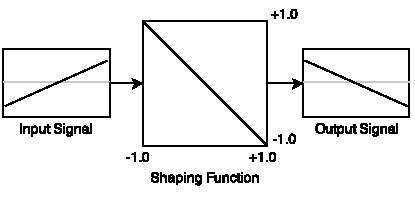
\includegraphics[width=0.75\linewidth]{images/waveshaping.pdf}}
  \caption[Using a waveshaping function to transform a signal -
  \protect\newline{\small based upon \cite[p. 255]{curtis1996computer}}]{Using a waveshaping function to transform a signal}
  \label{fig:waveshaping}
\end{figure}

The example in \reffigure{fig:waveshaping} shows a linear shaping function ($ f(x) = -x $) and a linear input signal. The output of the shaping function is an inverted input signal. For the purpose of simplicity, both, the input signal and the shaping function, are linear functions, but waveshaping is not limited to linear functions. In normal applications of waveshaping, the signal and the shaping function are non-linear. For faster computation, shape functions can be represented as in-memory look-up tables for values from -1 to 1. A typical application for waveshaping is the overdrive effect, which is well-known from the distorted sound of heavy guitar music.

In the Web Audio API there is a special node for waveshaping, the \code{Wave\allowbreak ShaperNode}. It uses a pre-stored wave function to shape the connected audio signal. The following example creates an overdrive effect and is taken from the \code{tuna} library\footnote{\url{https://github.com/Dinahmoe/tuna}, Dinahmoe, last checked on 20/03/2014}, which provides a variety of effects for the Web Audio API\footnote{For abbreviation, the part about loading and connecting a buffer, as seen in the examples before, is left out.}.

\begin{lstlisting}[language=JavaScript, caption=Using the WaveShaperNode, label=lst:waveshaper-node]
  var samples = 8192;
  var table = new Float32Array(samples);
  var amount = .7;
  var k = 2 * amount / (1 - amount),
      i, x;
  for(i = 0; i < samples; i++) {
    x = i * 2 / samples - 1;
    table[i] = (1 + k) * x / (1 + k * Math.abs(x));
  }

  waveshaper = context.createWaveShaper();
  waveshaper.curve = table;
\end{lstlisting}

For the representation of the curve, a \code{Float32Array} is used instead of a normal array (line 2, \reflisting{lst:waveshaper-node}), which is filled by iterating over the amount of \code{samples} (line 6) and calculating the function's value at the current point (line 8). In short, the above created curve table represents a variable version of the mathematical function $ f(x) = \frac{x}{abs(x)} $ which acts as a clipping function for the input signal. The clipping threshold is defined by the value of \code{amount} (line 3) and is typically a parameter that is defined by users.
%!TEX root = ../../thesis.tex

\section{Timing}
\label{sec:webaudio-timing}

\begin{quote}
  ``Silence is very important. The silence between the notes is as important as the notes themselves.'' - Wolfgang Amadeus Mozart
\end{quote}

One of the most important aspects of making music, no matter if it's digital or analogue, is timing. Songs are made of notes which are played at specific points in time. The gaps between the notes create a rhythm which plays a big role in the perception of songs. Only knowing about the individual notes of a composition is useless without having information about the rhythm and, therefore, about the timing.

\subsection{Timing methods in JavaScript}
\label{subsec:timing-in-js}

In JavaScript there are several ways to time code execution. The global method \code{setTimeout(func, delay)} \cite[chapter: setTimeout]{MDN} delays the execution of \code{func} by \code{delay} milliseconds. So, if an arbitrary function called \code{doIt} should be executed after one second, the code would look like this: \code{setTimeout(doIt, 1000)}. The execution of \code{func} can be prevented by calling \code{clearTimeout(timeoutId)} with the id that was returned by \code{setTimeout}.

Besides \code{setTimeout} there is also \code{setInterval(func, delay)} \cite[chapter: setInterval]{MDN} which will repeatedly execute \code{func} each time \code{delay} milliseconds have passed. In line with the above mentioned \code{clearTimeout\allowbreak (timeoutId)}, the execution of \code{func} can be prevented by calling \code{clearInterval\allowbreak (intervalId)}.

In theory, these methods could be used to properly time sounds and arrangements but they have some drawbacks. The JavaScript runtime does not guarantee that callbacks are called exactly at the specified point in time. Generally, the execution is off from the planned point in time by some milliseconds, even when there are no heavy computations on the website\footnote{\url{http://jsfiddle.net/janmonschke/sar5x/}, last checked on 10/03/2014}. The delay can even increase by several hundred milliseconds when there is user interaction like a window resize or a tab switch. In most browsers, interval times are also limited when the current tab becomes inactive. The Mozilla documentation states that in their implementation ``intervals are clamped to fire no more often than once per second in inactive tabs''\footnote{\cite[chapter: setInterval]{MDN}}. All these problems make the methods useless for the needs of precise audio timing. 

\subsection{Timing nodes in the Web Audio API}
\label{subsec:timing-in-web-audio}

Timing in the Web Audio API does not rely on any of the normal JavaScript timing methods. Each \code{AudioContext} has a \code{currentTime} property which returns the precise amount of seconds that have passed since the context has been created. This property can be used to time the beginning of a buffer or the beginning of an oscillator. As described in \refchapter{sec:webaudio-buffer}, buffers are started by calling their \code{start} method. The buffer's \code{start} method has three parameters: \code{buffer.start(when, offset, duration)}. \code{when} defines the point in time at which the buffer should be started, \code{offset} defines the amount of seconds that should be skipped and \code{duration} defines for how long the buffer should be played. The unit for all these values, as well as for all other values in the Web Audio API that deal with timing, is seconds. The oscillator's (\refchapter{sec:webaudio-osc}) \code{start} method only has a \code{when} parameter because \code{offset} and \code{duration} only make sense for nodes with a predefined length.

\begin{lstlisting}[language=JavaScript, caption=Usage of the start method's parameters, label=lst:currentTime]
  buffer.start(context.currentTime + 1, 2, 1);

  oscillator.start(context.currentTime + 1)
\end{lstlisting}

\reflisting{lst:currentTime} illustrates how to use \code{context.currentTime} in combination with the \code{start} method. Line 1 schedules a buffer to start in one second with a buffer-offset of two seconds and will end the playback after a duration of one second. Line 2 starts an oscillator in one second. It is important, that the \code{currentTime} is added to the \code{when} parameter, because the Web Audio API starts nodes by comparing the \code{when} parameter to \code{currentTime}. If only \code{1} were passed as the first parameter in line 1, it would not get scheduled to play in one second but at whatever point in time is defined by \code{currentTime - 1}.

To demonstrate how powerful the \code{start} method is, the following listings will show how to write a simple drum loop and a scheduler that only uses the \code{when} parameter.

A drum loop is a series of beats of which each represents an individual percussion instrument that is typically found in drum sets, such as a snare drum or a kick drum. The example loop has sixteen beats and consists of three different sounds (`hihat', `kick', `snare'). Scheduling the drum loop can be done with only a for-loop that iterates over the amount of beats. \reflisting{lst:drumloop} schedules a simple drum pattern that plays the hihat on every other odd beat, it plays the kick drum on beats one and nine and it plays the snare drum on beats five and thirteen.

\begin{lstlisting}[language=JavaScript, caption=Scheduling a simple drum loop, label=lst:drumloop]
  for(var i = 1; i < 17; i++){
    if(i % 2 == 1)
      play("hihat", i);

    if(i == 1 || i == 9)
      play("kick", i);

    if(i == 5 || i == 13)
      play("snare", i);
  }
\end{lstlisting}

The above example lacks some information on how the scheduling actually works. So far it only contains details about which note to play on which beat but no details about the speed, which is, as already described above, necessary to perform, or in this case to schedule, the song.

The speed of a song is often described in \emph{beats per minute (bpm)}. The \code{play} method in the next example only needs to know about the seconds between each beat to properly schedule a beat. As \reflisting{lst:rhythmscheduling} shows in line six, the scheduling of a sound is done by simply multiplying the index of its beat by \code{secondsBetweenBeats} which is calculated in line three from the \code{bpm} and the speed\footnote{Dividing (60 / bpm) by 4 creates the time in seconds between 16th notes.}.

\begin{lstlisting}[language=JavaScript, caption=Scheduling with a certain speed, label=lst:rhythmscheduling]
  var bpm = 120;
  var secondsBetweenBeats = (60 / bpm) / 4;

  var play = function(buffer, beat){
    var bufferNode = getBuffer(buffer);
    bufferNode.start(beat * secondsBetweenBeats);
  };
\end{lstlisting}

Of course, this scheduler is very limited because it is only capable of playing a drum loop once and there is no way to change the speed or the rhythm, but it is a good example that shows how a basic, precise scheduler can be implemented. \refchapter{sec:impl-scheduling} introduces a more complex and feature-rich scheduler that makes use of old (\code{window.setInterval}) and new (\code{node.start}) timing methods in combination.

\subsection{Timing parameters}

The Web Audio API also gives fine grained access to a node's parameters and allows for the ability to time and to interpolate them in various ways. Parameter values, however, cannot be changed directly but have to be changed by accessing a parameters's \code{value} property like so: \code{gn.gain.value = 1.2}. By using the GainNode's \code{setValueAtTime} method, this operation can be scheduled to a point in the future, e.g. \code{gn.gain.setValueAtTime(2, now + 1)} (assuming that \code{now = context.currentTime}) will set the gain to the value of two in one second from now.

In addition to that, a node's parameters can also be interpolated over time by using their \code{linearRampToValueAtTime} method: \code{linearRampToValueAtTime (2, now + 2)} will interpolate the gain's value linearly for two seconds, until it has reached the value of two. Nodes also have methods to interpolate parameters exponentially (\code{exponentialRampToValueAtTime}) and to interpolate parameters using a custom curve (\code{setValueCurveAtTime}) and their description can be found in the official Web Audio documentation\footnote{\url{http://webaudio.github.io/web-audio-api}, accessed 13.03.2014}.

These timing methods are all part of the \code{AudioParam} interface, which is used for all audio parameters, e.g., the oscillator's \code{frequency} parameter, the filter's \code{Q} parameter or the B\code{ufferSourceNode's playbackRate}. They make it much easier and much more accurate to control a node's behavior than it would be by using custom \code{window.setTimeout} handlers.

\subsection{ADSR Envelope}
\label{sec:adsr-envelope}

A perfect use case for parameter timing is the implementation of ADSR envelopes. ADSR is an acronym and stands for Attack, Decay, Sustain and Release envelope. It is a way of controlling the perception of a sound by dividing it into different phases which each have a different amplitude \cite[p. 97]{curtis1996computer}. When artists play a note on a piano, they have full control over how hard they push a key and therefore control over the attack of a sound, which, depending on the power that is used, can be louder than the rest of the sound. This effect cannot be reproduced with normal (digital) computer keyboards, because they can only be pressed or released. These keyboards can mimic the length of a sound. It might sound like a slight detail to influence the sound with ADSR envelopes, but it is actually a very common way to compose unique and distinguishable sounds.

\begin{figure}[htb]
  \centerline{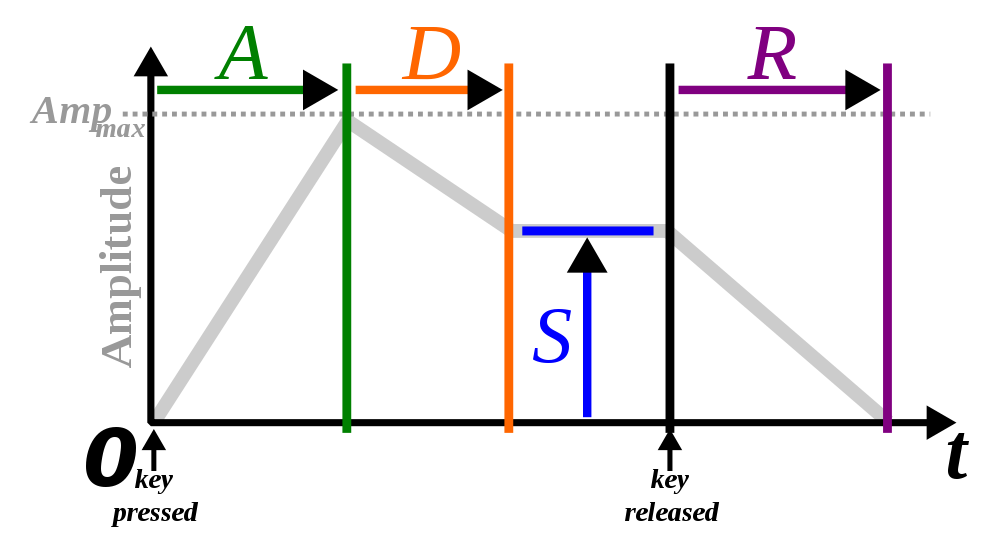
\includegraphics[width=0.8\linewidth]{images/ADSR_parameter.png}}
  \caption[Impact of an ADSR envelope on a sound's amplitude over time -
  \protect\newline{\small\url{http://commons.wikimedia.org/wiki/File:ADSR_parameter.svg} (01.23.2014)}
  \protect\newline{\small\emph{WikiMedia - User:Abdull}}]{Impact of an ADSR envelope on a sound's amplitude over time}
  \label{fig:ADSR}
\end{figure}

\reffigure{fig:ADSR} shows the four different phases of an ADSR envelope.

\begin{description}
  \item[Attack] \hfill \\
  The time it takes to reach the max level, starting from zero when the key is pressed.
  \item[Decay] \hfill \\
  The time it takes to interpolate to the sustain level.
  \item[Sustain] \hfill \\
  The normal amplitude level of the sound. Depending on the application, sustain either can be defined only as an amplitude level or the sustain property of an envelope can also contain duration information.
  \item[Release] \hfill \\
  Interpolation time to zero, starting from the sustain level when the key is released.
\end{description}

This concept gives us the option to control a sound like piano players (the piano pedal information is based on: \cite[p. 72]{pilhofer2011music}). The attack and the decay parameters correlate to the key pressure and the key speed. A shorter attack value leads to a sharper sound, whereas a longer attack value makes a sound softer. The sustain parameter, if it contains a duration information, is similar to the effect that is created by using the sostenuto pedal on a piano (middle pedal), it will sustain the sound until the pedal is released. Release time can be altered by using the damper pedal (right pedal), which will release the dampers and make the tones sound longer.

\begin{lstlisting}[language=JavaScript, caption=A minimalistic ADSR envelope in JavaScript, label=lst:adsrenvelope]
  var keydown = function(){
    var now = context.currentTime;
    buffer.gain.setValueAtTime(0, now);
    buffer.gain.linearRampToValueAtTime(maxLevel, now + attack); // ATTACK
    buffer.gain.linearRampToValueAtTime(sustainLevel, now + attack + decay ); // DECAY
  };

  var keyup = function(){
    var now = context.currentTime;
    buffer.gain.value.linearRampToValueAtTime(0, now + release); // RELEASE
  };

  document.addEventListener("keydown", keydown);
  document.addEventListener("keyup", keyup);
\end{lstlisting}

In \reflisting{lst:adsrenvelope}, a minimal envelope is implemented using the above mentioned timing methods. It assumes that \code{buffer} is a \code{BufferSourceNode} which is already loaded, that \code{context} is a \code{WebAudioContext} and that \code{maxLevel} and \code{sustainLevel} are predefined number values. The methods \code{keydown} and \code{keyup} are executed whenever their corresponding events are fired on the \code{document} object (lines 13--14). In \code{keydown}, the buffer's gain is set to zero initially (line 3) and then scheduled to rise up to the \code{maxLevel} value after the \code{attack} time has passed (line 4). Directly after that, the gain is scheduled to go down to the \code{sustainLevel} after the decay time has passed (line 5). On first sight, it might look wrong to schedule two linear interpolations at the same time, because they would interfere with each other if they were run simultaneously. In the Web Audio API, however, all scheduling methods are executed consecutively for each parameter so that two scheduled events on the same parameter cannot interfere \cite[Chapter 4.5.2.]{wilson2014webaudiospec}. In the example above, it means that the decay-interpolation is not triggered until the attack-interpolation finished. When a key on the keyboard is released, the \code{keyup} handler will interpolate the buffer's gain to zero for as long as \code{release} was set (line 10). 
%!TEX root = ../../thesis.tex
\section{Synthesizers}
\label{sec:webaudio-synth}
\begin{quote}
  ``I knew that it could be a sound of the future but I didn't realise how much the impact would be.'' - Giorgio Moroder
\end{quote}

The term `synthesizer' describes music instruments that create sounds solely electronically. The term was coined in the late 1960s by Robert A. Moog, founder of Moog Music the pioneering company in the field of analog synthesizers \cite[p. 67]{pinch2004analog}. Moog decided to call it `synthesizer', although the term was used before for another instrument, the `RCA synthesizer' which was also used to synthesize sounds, but which did not have the ability to be played in real-time, it needed to be programmed\footnote{\cite[p. 67]{pinch2004analog}}. Moog's synthesizers were modular synthesizers, meaning they consisted of individual modules that had to be patched together with wires in order to route the audio signal through filters and envelopes before it was sent to the speakers. The sound was created from electronic oscillators which were triggered by a keyboard that was attached to the synthesizer\footnote{\cite[p. 25ff]{pinch2004analog}}. Synthesizers were made famous in popular music in the 1970s by acts like Kraftwerk and Giorgio Moroder, who wrote the possibly most famous synthesizer-based song of that time: `I Feel Love' performed by Donna Summer \cite[14:37min]{bbc2009synthbritannia}. Since the first introduction of synthesizers in the 1960s, their architectures changed a lot and in addition to analog synthesizers, digital synthesizers and software synthesizers have been introduced. Today, synthesizers build the foundation of modern electronic music and they can be found in all DAWs.

There are many different ways how synthesizers can be implemented and they base on different theoretical approaches. This chapter will however focus on the background theory of analog synthesizers and only mention other approaches briefly.

Analog synthesizers, such as the ones that were created by Moog (Minimoog, Moog Modular etc.), are based on the concept of `subtractive synthesis'. In `subtractive synthesis', rich audio signals are taken and then manipulated to make them sound `less rich'. `Less rich' in this context does however not mean that the sound signal becomes less appealing to listeners. It means that the spectrum of the signal is reduced and that certain parts are emphasized, while other parts are left out \cite[p. 223f]{park2009introductionto}. The concept of the `subtractive synthesis' stands in contrast to the `additive synthesis', in which simple signals are added up to produce a more rich sound\footnote{\cite[p. 277f]{park2009introductionto}}.

\medskip

\begin{figure}[htb]
  \centerline{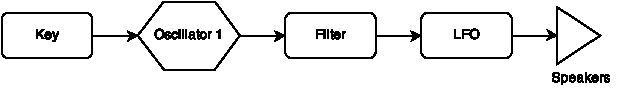
\includegraphics[width=\linewidth]{images/SimpleSynth.pdf}}
  \caption[A simple synthesizer's node graph]{A simple synthesizer's node graph}
  \label{fig:simple-synth-node-graph}
\end{figure}

The simplified node graph in \reffigure{fig:simple-synth-node-graph} shows how the signal's `richness' is shaped by the  different components of a synthesizer. The source of the signal is a raw oscillator (see \refchapter{sec:webaudio-osc}) signal which is initialized by pressing a key on the keyboard. Typically, a module that translates keys, which of course stand for musical notes, to the corresponding frequency lies in between the key and the oscillator. The oscillator's signal is then altered by a filter (see \refchapter{sec:webaudio-filter}) in order to remove some frequencies and in order to emphasize certain other frequencies. Next, the signal is routed into a Low Frequency Oscillator (LFO). The LFO's signal is used to modulate the amplitude or the pitch of the incoming signal in order to produce an alternating sound signal. The impact of this effect is determined by the LFO's frequency, which typically lies at the lower end of the human hearing. Humans would not be able to hear signal with this frequency, but the modulation of the input signal makes the alternations audible. The resulting signal is then routed to the speakers or to an audio-out port.

All parts from the above explained node graph can be implemented by using the Web Audio API's building blocks and build on top of them. \refchapter{impl-synth} will show which parts of the API could be reused and which could be combined to implement a synthesizer for the audio editor.

\chapter{Synchronization}
\label{ch:sync-theory}

%!TEX root = ../../thesis.tex
\section{Overview}

This chapter gives an overview of various techniques that ensure consistency in interactive collaborative environments with shared documents. These techniques will be rated based on their features (\refchapter{sync-features}), complexity and impact on the user experience (\refchapter{sync-ux}). In \refchapter{sync-discussion} one of the detailed techniques is picked for the implementation of the collaborative music editor by incorporating the evaluations that were formulated in this chapter. The selection of algorithms used in this chapter is, of course, not complete and all peer-to-peer syncing mechanisms have been omitted. This is due to the P2P stack that is available in modern web browsers (WebRTC) not currently being stable enough for such an important foundation of a web application. All shown techniques assume that the system underlies a client-server architecture.

\section{Features}
\label{sync-features}

Distributed collaborative systems allow users to work on the same documents\footnote{Document here, is seen as a general type of data and not as a text document, although a text document is used in most examples for simplicity.} at the same time. A variety of algorithms and techniques have been developed that enable simultaneous editing. According to \cite{sun1998achieving}, these all need to feature solutions to the three main inconsistency problems that occur in shared environments.

\subsection{Convergence}

Since document operations are executed locally, all local documents can be in a temporary state of divergence\footnote{\cite[p. 65]{sun1998achieving}}. This is acceptable, as long as the algorithm is capable of producing identical documents once all local changes are propagated throughout the entire system.

\subsection{Intention preservation}

Each local change to a document has a certain intention. This `local' intention needs to be preserved when an operation is executed on other remote documents\footnote{\cite[p. 66]{sun1998achieving}}.

The impact of ``intention violation'' can be seen by evaluating concurrent edits to a text document (\reffigure{fig:OT}). Both users start off with the same document and edit the document simultaneously. They then send the changes to their other peer who subsequently applies those changes to his document. However, since the local document has changed, applying the other peer's alterations results in having a different document because the local intention of the action has not been preserved.

This feature might look similar to ``Convergence'', but it actually relates to a different problem. Convergence without Intention Preservation only ensures, that all participants have an identical document. But it is possible that this document can be the wrong document because the local intention was not preserved when the actions were applied.

\subsection{Causality preservation}

Every local operation is the result of the merge of all its previous operations, whether local or remote. Either way, each operation has a causal relationship to its predecessor. In distributed systems, messages arrive asynchronously and therefore they ``may arrive and be executed out of their natural cause-effect order''\footnote{\cite[p. 65]{sun1998achieving}}. For example, a user might receive an update of a value of an object, but the user has not yet received information about this object because the message has been delayed.

A common method to tackle this problem is to delay the execution of operations until their causal predecessors have arrived. \cite[p. 2ff]{fidge1988timestamps}

\section{User Experience}
\label{sync-ux}

In terms of user experience, the algorithm should permit a document to be edited locally. Clients should not need to wait for merged documents from a server while not being able to perform another operation on the document. Due to the latency of distributed systems, users will certainly see a delay between their actions and the visual feedback, leading to annoyance and irritation. The technique needs to support \textbf{Latency Hiding} in order to provide a good user experience.

Considering that a lot of users edit a document concurrently, the algorithm needs to merge a great deal of interdependent changes. This may result in cases that are not mergeable, in which case certain actions cannot be respected. These cases need to be detected and taken care of. The system should not simply fail silently and then report when it failed. The required features according to this problem can be described as \textbf{Graceful Exit}.

In addition to the above, the system should allow every user to edit the entire document at any given time. It should not matter how many users are connected to the system, nor which part of a document is being edited, nor should it matter by which user is being edited. If all this is achieved, the algorithm supports \textbf{Full Concurrency}. Not having Full Concurrency may lead to frustration in collaborative environments because users can block the work of other users.
%!TEX root = ../../thesis.tex
\section{Locking}
\label{sync-locking}

\begin{figure}[htb]
  \centerline{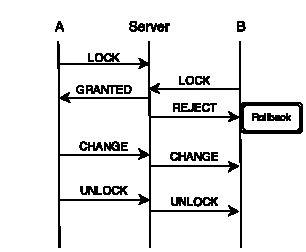
\includegraphics[width=0.65\linewidth]{images/Locking.pdf}}
  \caption[Communication in a locking algorithm]{Communication in a locking algorithm}
  \label{fig:Locking}
\end{figure}

Locking algorithms, often also referred to as `pessimistic' algorithms, define a system in which only one user is allowed to edit a document with simultaneous edits being forbidden \cite[p. 2]{fraser2009differential}. When starting to edit a document, the client sends a LOCK request to the server that can either be granted or rejected due to another client previously locking the document (see \reffigure{fig:Locking}). In case of a rejection, the client will have to rollback the changes that have been made during the time of the ongoing LOCK request \cite[p. 5]{sun2002locking}. The client that locked the document is allowed to send CHANGE packets to the server, which in turn propagates to all other connected clients. Likewise, when the document is unlocked, the UNLOCK packet is sent to all other peers.

When a locking algorithm is correctly implemented, it disallows simultaneous edits to the same document and therefore fulfills all three major features of a synchronization algorithm. Nevertheless, the locking has a negative impact on the user experience because users cannot edit the document while it is being locked. In addition, a locking system is not consistent during a packet loss. When an UNLOCK packet does not reach a user, its document will be locked indefinitely, unless the client polls the lock state. Another problem occurs when a LOCK packet is lost. A user might make significant changes to a document, not knowing that it is locked. When the client then tries to send the changes to the server, it will be blocked and all changes need be removed.

Instead of locking the whole document, \cite[p. 5ff]{sun2002locking} proposes a fine-grained locking mechanism which results in a better user experience. Given that only parts of a document can be locked users can work on the same document simultaneously. Yet still, this does not allow all users to edit the complete document at the same time and consequently does not meet the requirement of \textbf{Full Concurrency}.
%!TEX root = ../../thesis.tex
\section{Three-way merges}
\label{sync-3waymerges}

\begin{figure}[htb]
  \centerline{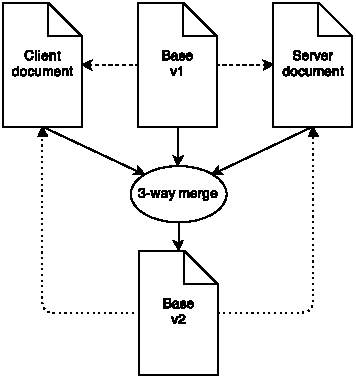
\includegraphics[width=0.55\linewidth]{images/Three-way_merge.pdf}}
  \caption[Illustration of a three-way merge - based upon
  \protect\newline{\small\url{https://neil.fraser.name/writing/sync/3way.gif} (02.5.2014)}
  \protect\newline{\small\emph{Neil Frasier}}]{Illustration of a three-way merge}
  \label{fig:Threewaymerge}
\end{figure}

Three-way merges are commonly used in many source code management systems, e.g. in git \cite[p. 52]{scott2009pro} or in CVS \cite[p. 31f]{lindholm2001athreeway}. Their purpose is to allow users to work on the same files simultaneously without necessitating a constant connection to a server. The way a three-way merge works is illustrated in \reffigure{fig:Threewaymerge}. The algorithm takes the changed local version of the document, its base version and the changed server document (that is also based upon the same document as the client's). It then compares the changes that were made to both new documents, in comparison to the base version \cite[p. 2f]{mens2002softwaremerging}. These changes are then merged into a new version of the document, on which all subsequent changes have to be built on top of. Sometimes not all changes can be merged into a new version automatically e.g. because both changed versions have alterations to the same part of the document. This results in a conflict that can only be resolved manually by the user, which is one of the reasons why three-way merges are often executed on the client.

This approach can also be used for real-time collaborative editing by permitting clients to send their new versions of the document to the server, which then performs a three-way merge and returns the newly generated base document or the list of conflicts that the user needs to resolve \cite[p. 220ff]{minor1993semiasynchronous}. In this way, all users could edit the same document(s) simultaneously. Since all edits are done locally and all conflicts need to be resolved manually, this algorithm ensures that Convergence, Intention Preservation and Causality preservation are achieved. Furthermore, it complies with the UX requirements: \textbf{Graceful Exit} (manual conflict resolution) and \textbf{Full Concurrency} (documents are not locked). 

One major drawback to this technique is that it is poor at Latency Hiding. This is due to the fact that no updated document can be sent to the server while the user is editing. Once the user has finished, an updated version can be sent and merged but if the document has been updated during the merge, the merged version cannot be applied and needs to be revoked \cite[p. 2]{fraser2009differential}. This behavior results in versions that will diverge more over time, thus generating a higher chance for merge conflicts and merge conflicts require user interaction. Having to deal with merge conflicts instead of being able to focus efforts on working on the document has a bad impact on the user experience.

In addition to this, the algorithm does not scale well for larger documents, as the whole document needs to be transferred to the server for each merge. Also it does not scale in scenarios with many connected users. This is due to the problem that having more simultaneous users in a system, the chances of merge conflicts rise.
%!TEX root = ../../thesis.tex
\section{Operational Transformation}
\label{sync-ot}

Operational Transformation (OT) was introduced by \cite{ellis89groupware} and resulted from their work on a groupware editor called Grove. Their technique is used in many web-based collaborative editors e.g. in Google Docs and Etherpad \cite{lautamaki2012cored}. A lot of research has been done on the topic since the original paper was issued. OT bases itself on the idea of sending operations on documents to a central server, which in turn propagates operations to all other peers. An operation is defined as a tuple of fine-grained changes to a document which contains information about the intention of the change (e.g. delete, insert), the position of where to apply the change in the document and a sometimes optional value for the change. Given the text ``HTW'', the operations \emph{O\textsubscript{1}=insert[0, ``F'']} and \emph{O\textsubscript{2}=delete[1, 1]} will result in the new text ``FTW''.

Each client in the network begins with the same document and from then will only send and receive operations on that document, updating the original itself. In that way, the network traffic is kept to a minimum and the server work is reduced because clients merge operations themselves. However, this architecture and the latency of the transport medium (nowadays the Internet) cause problems when operations overlap:

\begin{figure}[htb]
  \centerline{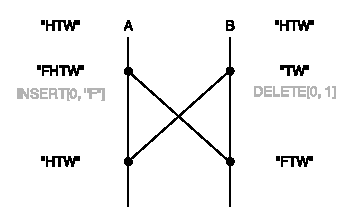
\includegraphics[width=0.8\linewidth]{images/Operational_Transformation.pdf}}
  \caption[Overlapping Operations in OT - based upon
  \protect\newline{\small\cite{nichols95jupiter}}]{Overlapping Operations in OT}
  \label{fig:OT}
\end{figure}

Client A and Client B both insert a character into the document at the same position, at the same time. The resulting text for Client A is now ``FHTW'' and the text for Client B is ``TW''. Both changes are sent to the other peers (a communication server is left out in the diagram) where they are applied to the local documents. When Client A applies the operation to the document it generates ``HTW'', but when Client B applies it to the document, the resulting text is ``FTW'' meaning that both documents diverge and the intentions of the original operations are not preserved.

A proposed solution from the original paper is to delay the execution of operations until they are executed in the correct order and, if the operations contain overlapping changes, to transform the operations in a way so that they preserve the original intention (dOPT\footnote{\cite[p. 403f]{ellis89groupware}}). The solution in its original form was limited however to P2P connections, divergence of just one step and was proven to be incorrect by \cite{cormack1995counterexample}. 

Another solution for a ``concurrency control'' system was described by \cite{nichols95jupiter} and is derived from their work on a multi-user multimedia collaboration tool named Jupiter. Instead of allowing peers to exchange their operations directly, their approach is to put a synchronization server in between, thus taking care of broadcasting the changes to all clients. In their algorithm, the transformation of operations is handled on the client and the server. When clients receive an operation that conflicts with their own last operation, they create a transformed operation from a \code{transform()} method for which the following needs to apply: $C' * S = S' * C$, where $C$ is a client operation, $C'$ a transformed client operation, $S$ a server operation and $S'$ a transformed server operation \cite[6:30min]{whitelaw2009ot}. Fundamentally this means, that client and server are capable of reaching identical documents by resolving operation conflicts on their own sides and therefore \textbf{Convergence} is guaranteed.

Since the release of the original research papers, there have been a number of papers introducing new algorithms that improve OT's characteristics and lead to more stable systems that also comply with \textbf{intention preservation} and \textbf{causality preservation} e.g. \cite{sun1998achieving} and \cite{wang2010wave}. 
Yet, most OT implementations are based on a combination of many different algorithms, chosen dependent on the system's requirements. This makes the implementation of an OT system both non-trivial and time-consuming, a common critique of OT \cite{gentle2011sharejs}.

By design, OT fulfills all User Experience requirements because it allows clients to edit the document locally (\textbf{Latency Hiding}), yet does not lock the document or parts of the document (\textbf{Full Concurrency}) and has the capability of detecting and handling diverging documents (\textbf{Graceful Exit}).
%!TEX root = ../../thesis.tex
\section{Differential Synchronization}
\label{sync-diffsync}

\begin{figure}[htb]
  \centerline{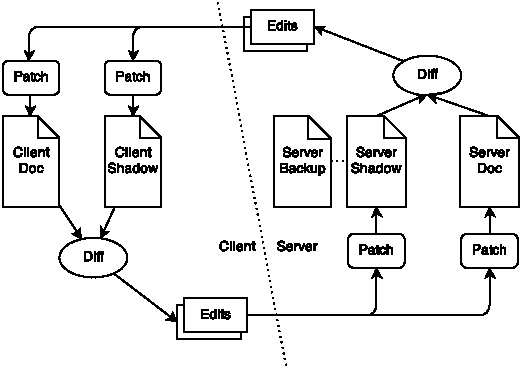
\includegraphics[width=0.8\linewidth]{images/Differential_Synchronization.pdf}}
  \caption[Illustration of Differential Synchronization - based upon
  \protect\newline{\small\url{https://neil.fraser.name/writing/sync/diff3a.gif} (02.5.2014)}
  \protect\newline{\small\emph{Neil Frasier}}]{Illustration of Differential Synchronization}
  \label{fig:DiffSync}
\end{figure}

Differential Synchronization (DS) is based on similar techniques that are also used in the Three-way merge algorithm (see: \refchapter{sync-3waymerges}). As a result of its highly different architecture, it is also suited for real-time collaborative editing. The algorithm, introduced by \cite{fraser2009differential},  has shown that it is stable and well-suited for interactive applications \cite[p. 8]{koren2013sharedediting}, despite the fact that it is a young algorithm in comparison to \refchapter{sync-ot}.

Server and client start off with an identical version of the document and then both create a copy of that document which will work as the shadow document of the client and as the shadow document of the server respectively. These shadows will always contain the state of the document that lies on the other end. As shown in \reffigure{fig:DiffSync}, the synchronization sequence is always initiated by a change of the document by a client. This change will trigger the creation of a diff between the local copy and the client shadow which is then added to the local stack of edits. A message that contains the newly created diff and metadata, such as checksums and version numbers, is built and sent to the server. The diff that is contained in the message is then patched to the server shadow (which represents the current state of the client) and the outcome is then compared to the checksum that was previously transmitted alongside the diff. If the checksum matches, the diff will also be applied to the server's copy of the document and the old version of the server shadow will be copied to the backup shadow. If the checksum does not match, the diff has been corrupted during transmission, which means the client needs to refetch the document and throw away the diff. Subsequent to patching the server's documents, a diff is created from the recently patched documents (shadow and server copy). This diff will include changes that were made to the document by other peers in the network. An edit message is created on the server and sent to the client, who then patches and diffes these changes again, in the same way as the server previously did.

The above process is restricted to one simultaneous request per user at one time in order to preserve consistency. Users are still permitted to edit the client's document during a request, but the changes will only be sent to the server after the last request been processed. In this way, DS ensures \textbf{Full Concurrency} and provides a mechanism of \textbf{Latency Hiding}.

DS is capable of handling packet losses for both requests and responses. By comparing version numbers of each edit on server and client and by keeping a stack of edits, the algorithm is able to detect and handle inconsistencies. If for example, a packet is lost on its way to the server, its edit will be sent the next time the client wants to send an update. This is because the client's edit-stack is only reset if it receives an edit from the server that contains the merge of the last edit. Since the server did not receive the last edit in this case, it did not send another edit to the client and the client's edits-stack is not emptied\footnote{\cite[p. 4]{fraser2009differential}}.

When a packet gets lost on its way to the client, the next client-request will contain incorrect version numbers and the server will load the backup shadow (which always represents the version before the last successful patch) into the server shadow. It will apply the edits to the backup document, because the version numbers will match this document. In this case, the server will need to throw away its edit stack, because the edits are now based on different versions, and will therefore only send a diff from the newly patched document.

A key factor of DS is the implementation of the diff and patch actions, which greatly depend on the underlying data structure. The diff implementation needs to have a high performance, because it could be executed several times a second, dependent on how often the client initializes a sync request. The patch implementation needs to be fuzzy, meaning it should be able to incorporate changes to documents that might have diverged over the course of several seconds. The fuzzy implementation should merge the diffs in way that it respects the semantics of the data structure. Diff and patch being the key factor of DS also means that it is agnostic to data structures. DS can be applied to all data structures that have adequate implementations of patch and diff\footnote{\cite[p. 5]{fraser2009differential}}. The combination of diff and patch is responsible for \textbf{Convergence} and \textbf{Intention Preservation} of the algorithm. The overall architecture of the technique ensures, that no document can reach a state where the causality of actions is violated, thus guaranteeing \textbf{causality preservation}\footnote{\cite[p. 1]{fraser2009differential}}.

The client should ensure that synchronization cycles are initiated more often than there are changes on the document. This is because a user may not edit the document for a while and in this time he will not receive updates from other collaborators due to the asynchronous nature of the initialization process. In addition to document changes, the synchronization process should get triggered at certain intervals to make the application seem more interactive \cite{instantSyncThesis}. The less time there is between synchronization cycles, the better will the diff and patch actions perform and the better will the algorithm perform in providing \textbf{graceful exit} methods. This is down to the fact that there will be smaller changes and therefore less contextual changes, which then leads to fewer conflicts in the document. This also implies that when a packet is corrupted during transmission, as described above, the system will lose only little information.

Although DS is based on a client-server architecture, it could also easily be adapted to make it usable in peer-to-peer networks. In this scenario all participants would be able to send their local changes to other peers, requiring each client to also have a backup document for every other peer in the network\footnote{\cite[39:20min]{fraser2009video}}. This makes the implementation of client and server even more analogue, since every client is now essentially a server in its own right.

% State transfer vs. operation transfer
% \cite{saito2005optimistic}
%!TEX root = ../../thesis.tex
\section{Discussion}
\label{sync-discussion}

All four discussed algorithms and techniques meet the required features that were described in (\refchapter{sync-features}). Their main differences lie in the fulfillment of the user experience requirements.

Locking does not allow users to edit the entire document simultaneously and is therefore unsuitable for the purpose of the music editor. When it comes to composing synthesizer arrangements, collaborative editing provides an advantage because both users can immediately correct mistakes or improve the harmony of a melody.

Although three-way merging does permit users to simultaneously edit the entire document, it does have the drawback of confronting users with merge conflict dialogs and as well as having a lack of real-time updates whilst users are editing themselves. A collaborative work on synthesizer arrangements could lead to many merge conflicts and in addition, users would not see other users' changes whilst editing.

Operational Transformation not only complies with all required features but also complies with the User Experience requirements. Nonetheless, it still has some drawbacks. Firstly, it is difficult to gain an overview of all available algorithms, techniques and their disadvantages because the topic has been researched for so many years, which makes finding the right combination of solutions really hard. Secondly, once decided upon which techniques to use, implementing a failsafe OT system from scratch would take up a great deal of time. Joseph Gentle, former Google Wave\footnote{Google Wave, now known as Apache Wave, is a collaborative multimedia communication tool which used OT to enable real-time editing} engineer, said: ``Wave took 2 years to write and if we rewrote it today, it would take almost as long to write a second time.''\footnote{\cite{gentle2011sharejs}}. Lastly, all papers were only using text documents and their basic operations (e.g. insert and delete) to describe their algorithms. The editor that will result from this thesis will be based on JSON objects. Thus, a large set of new operations would need to be created and tested. The amount of work that is required for this would be a thesis in itself.

Differential Synchronization also complies with both required features and user experience requirements but is, in comparison to OT, much easier to implement as it can be based on existing diff- and patch algorithms. Once again, the original paper only presented solutions for dealing with text documents but the algorithm works independently from the underlying data structures. The only limitation is that the data structure needs to have a suitable diff and patch implementation (which will be shown in \refchapter{impl-sync-algorithm}). All aspects considered, DS appears to be very well-suited for the purpose of a collaborative music editor and is therefore chosen in favor of OT. Currently there are no implementations of this approach where both server and client are written in JavaScript and the base data structure is a JSON document. The implementation of the music editor based on DS in JavaScript would advance the research on DS in general.

\chapter{Realtime Technology}
\label{ch:realtime-theory}

%!TEX root = ../../thesis.tex
\section{Overview}

Websites have become highly interactive and contain more collaborative features which are enabled by new ways of client-server and client-client communication. In many use-cases it is no longer sufficient to simply display static sites, because other users may already have edited the content on these sites and the displayed information is rendered outdated. Clients need to be notified about these changes and reload parts of the website so that the displayed information matches the most recent version of the data.

This chapter will give an overview of old and new techniques for data exchange. Both their advantages and disadvantages shall be discussed in order to evaluate which technology will be used in particular parts of the implementation of the collaborative editor.
%!TEX root = ../../thesis.tex
\section{XHR Polling}

A simple method to check if there is new data on the client is to ask the server at certain intervals if it has new data for the client (``Polling''). The XMLHttpRequest\footnote{XMLHttpRequest is a technique that allows clients to send HTTP requests to servers. Although it has `XML' in its name, it actually supports arbitrary data formats. It is the most common way to request data in modern web clients.}(XHR) is the main data exchange technology used for this purpose. Sometimes, especially when it involves external APIs or legacy clients that do not support XHR, JSONP\footnote{JSONP is a technique to request data from servers by creating script-tags with a specific url. The server will then return JSON data encapsulated in a global callback function. Since there is no way to check if malicious code is being sent, this technique is considered insecure.} is used in its place but it is a limited, as well as insecure, way of handling client-server communication and is thus disregarded in this comparison.

\begin{figure}[htb]
  \centerline{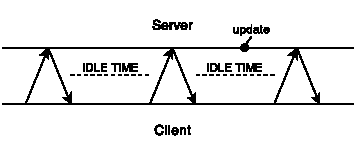
\includegraphics[width=0.8\linewidth]{images/Polling.pdf}}
  \caption[XHR Polling communication]{XHR Polling communication}
  \label{fig:polling}
\end{figure}

The simplest case for polling data from the server is shown in \reffigure{fig:polling}: the client periodically checks for new data on the server. If new data is received, it will be used to display the updated content. Afterwards, the client schedules a new request. The limitations of polling can easily be seen even from a simple example as presented in the figure above. The client will never receive updates in real-time and has a worst-case delay of IDLE-TIME. It should also be considered that there could be a large number of concurrently connected clients, all of whom request data at the same time interval. The server would need to handle request peaks in these intervals. Another weakness of polling is that it creates a traffic overhead by initiating too many unneeded requests.

One method to overcome some of these problems is to adapt the polling interval based on both the results of the first requests and the semantics of the requested information \cite{wanstrath2009pollinginterval}. If the requested information is based on an operation that needs a long time to finish, the polling interval could be adjusted to lengthen after each request. This would lead to fewer client requests and accordingly fewer request peaks. Yet still, this technique does not enable real-time updates.

\begin{figure}[htb]
  \centerline{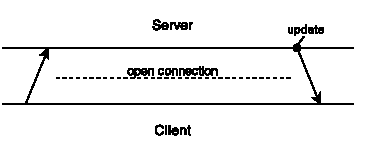
\includegraphics[width=0.8\linewidth]{images/Long_Polling.pdf}}
  \caption[XHR long polling communication]{XHR long polling communication}
  \label{fig:longpolling}
\end{figure}

An improvement to the standard polling mechanism is called long polling \cite[p. 276]{grigorik2013high}. Instead of asking for updates at a certain interval, clients connect to a server that will maintain an open connection until there is an update on the requested resource. The duration of the open connection from the client to the server is limited by a browser-specific timeout (circa 1-2min) but it is still much higher than the time between requests that is needed in classic polling. The typical connection flow of long-polling is shown in more detail in \reffigure{fig:longpolling}. Clients stay connected either until they time out or until the server responds with an update. Then they reconnect immediately after an update or a timeout.

This resolves some of the problems that occur with normal polling. Since clients timeout in different intervals, dependent on the browser vendor and the time of the update, servers will not have to handle request peaks. Through a reduction in the number of requests there is a significant decrease in traffic load on both sites, creating a much more efficient connection. Finally, updates occur in near real-time. The have a worst delay time of the amount time it takes to reconnect to the server.
%!TEX root = ../../thesis.tex
\section{Server-Sent Events}
\label{realtime-sse}

The Server-Sent Events API (SSE) is a standardised method to stream events from the server to the client. All events are sent via an open HTTP connection which makes the protocol very efficient and easy to optimise. \cite{hickson2012}

\begin{lstlisting}[language=JavaScript, caption=Messages in the Server-Sent Event protocol, label=lst:eventsource]
  data: { test: true }

  event: name
  data: { user: "test" }

  retry: 1000

  id: 3141592653589793
\end{lstlisting}

Messages in SSE require a special format, as shown in \reffigure{lst:eventsource}. Data messages must be prefixed by `data:' and they can be associated with a specific event by adding an `event:'-prefixed line above. As well as data messages, there are two additional control messages. The `id:' message in line eight represents the id of the last event that has been sent. In the case of a reconnect, this id would be sent to the server so that only events after this specific event would be sent to the client. Besides this, there are also `retry:' messages that specify the timeout time for the client before reconnecting to the server if the connection has been lost. \cite{bidelman2010sse}

\begin{lstlisting}[language=JavaScript, caption=Listening to server events in SSE, label=lst:eventsource-client]
  var source = new EventSource("/sse");

  source.onmessage = function(event){
    console.log(event.data);      // -> "{ test: true }"
  };

  source.addEventListener('name', function(event){
    var jsonData = JSON.parse(event.data);
    console.log(jsonData.user);   // -> "test"
  });
\end{lstlisting}

Clients simply have to connect to the server's ``EventSource'' and all events that are sent from that source will trigger DOM events from the connection object. \reflisting{lst:eventsource-client} demonstrates how to listen to events triggered by the two different message formats. Messages without event context (line 1 in \reflisting{lst:eventsource}) trigger the \code{onmessage} handler, whilst messages with event context (line three in \reffigure{lst:eventsource}) trigger listeners that have been added by \code{addEventListener}. The event object that is being transmitted to the listeners contains the message's content in its \code{data} attribute. This attribute is always interpreted as a String and therefore needs to be parsed if another format (e.g. like JSON in the above examples) has been used.
%!TEX root = ../../thesis.tex
\section{WebSockets}
\label{realtime-ws}

Websockets (WS) is a technology that adds a full-duplex\footnote{Full-duplex means that both sites are able send messages simultaneously.} communication channel between browser and server. WS stands for two things: 1) the WebSocket protocol itself and 2) the WebSocket API, an interface in the browser. The WS protocol has been designed to work as a general communication protocol and is not limited to a client-server scenario.

\begin{figure}[htb]
  \centerline{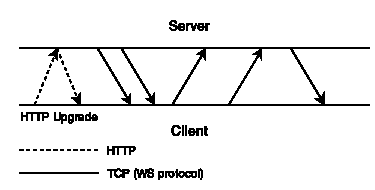
\includegraphics[width=0.9\linewidth]{images/Websockets.pdf}}
  \caption[Websocket communication]{Websocket communication}
  \label{fig:websockets}
\end{figure}

\reffigure{fig:websockets} shows the communication structure of a WS connection. All data is sent through an open TCP connection that is created after an initial handshake and negotiation through a HTTP Upgrade request from the client. This negotiation does not strictly rely on HTTP as handshake protocol but must be used by browsers as there is no browser API to create a TCP connection. In alternate setups (e.g. server to server WS), the negotiation can be based on any protocol, yet using HTTP has additional advantages. When HTTP is used for the handshake, it can be assured that WS works in any environment that is capable of using HTTP. Therefore both sides can use port 80 for the communication (respectively port 443 for secure connections) which are not blocked by most firewalls \cite[p. 298f]{grigorik2013high}. This enables developers to use WS in a variety of already existing environments without the need of altering firewall settings. The socket negotiation includes the exchange of environment keys, lists of supported protocol extensions and subprotocols as well as the protocol version. Once the handshake is complete, both sites can send and receive messages through the TCP connection. Messages do not require a request/answer pattern as with HTTP and can be sent asynchronously. This makes applications flexible and fast but also requires developers to adapt to a fully asynchronous message protocol \cite[chapter: Use Cases]{ubl2010websockets}.

\begin{lstlisting}[language=JavaScript, caption=Connecting to and using Websockets, label=lst:websockets]
  var ws = new WebSocket("ws://myserver.com/websocket");
  
  ws.onopen = function(){
    // connection established
    ws.send("hello server");
  };

  ws.onmessage = function(event) {
    console.log("new message", event.data);
    ws.close(); // ends the connection
  };

  ws.onerror = function(event){
    console.log("something went wrong", event);
  };
\end{lstlisting}

The browser's WS API is simple to use because it hides most of the protocol's complexities from the developer. Creating a WS connection to a server does not require a manual HTTP Upgrade request. It is entirely handled by the \code{WebSocket} object and its constructor as shown in \reflisting{lst:websockets} (line 1). All events trigger the attached event handlers in the same way that, say, DOM events trigger their events, so developers can use the same patterns here. The \code{onopen} trigger (line 3ff) informs the client that the connection has been established and it is now possible to send and receive messages. A client can send messages with the WS object's \code{send} method. The plain WS protocol does not support named message events like the SSE (see \refchapter{realtime-sse}) but they can be added manually by including the name of the event into the message itself. Once again, the WS object abstracts greatly from the WS protocol because messages are internally sent as so-called ``frames'' instead of simple strings. Frames are binary messages that encapsulate the data and contain the meta information of the messages (e.g. the length)\cite[p. 43ff]{wang2013websockets}. However, there is no way to reach to the frame level through the browser WS API.

The \code{onmessage} handler (line 8ff) is triggered when a server message arrives at the client. The \code{event} object, which is passed to the handler as the first parameter, contains the message content in its \code{data} property. If an error occurs somewhere in the communication, the \code{onerror} (line 13ff) handler is executed and more details about the error are handed in via the event object, so developers can react to any problem appropriately.

One advantage of WS over SSE, aside from supporting full-duplex communication, is its capability to send binary data. This means that client and server could use a fully custom protocol that is optimized for the specific use case of the application. In general, client and server have to agree on a custom protocol because there are no standardized messages or idioms like REST for the communication. However, WS was not introduced to replace XHR, which remains the first choice for web developers when it comes to data exchange with a server. WS was built for modern web applications with the need for push notifications or real-time communication in addition to normal HTTP requests.
%!TEX root = ../../thesis.tex
\section{WebRTC}
\label{realtime-webrtc}

WebRTC, short for Web Real-Time Communcation, is a new web communication technology that enables peer-to-peer multimedia broadcasting (audio, video and arbitrary data). It is being standardized by both the W3C\footnote{\url{http://www.w3.org/TR/webrtc}} and the IETF\footnote{\url{https://tools.ietf.org/wg/rtcweb/}} and, although it is already available in recent Chrome and Firefox versions, its API and the protocol are still in flux. The goal of WebRTC is not only to bring peer-to-peer multimedia streams to the web but also to act as a bridge technology to existing real-time applications so that browsers will be able to act as natural peers of these systems \cite[p. 310ff]{grigorik2013high}. This creates a broad spectrum of applications for WebRTC but it also renders it very complex. This section will omit many details that would be necessary to fully set up a WebRTC system but the complexity of such a system would go beyond the scope of the goal of this chapter. Therefore, it will focus on the usage of the client-side API and only briefly mention the possible network topologies and the various utilized protocols instead of explaining them all.

\begin{figure}[htb]
  \centerline{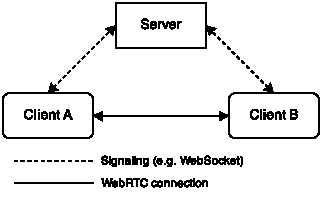
\includegraphics[width=0.9\linewidth]{images/WebRTC_connection.pdf}}
  \caption[A basic WebRTC setup]{A basic WebRTC setup}
  \label{fig:webrtc}
\end{figure}

In the most basic use case WebRTC can be used to establish a `phone' call between two parties (see \reffigure{fig:webrtc}). One of the parties (Client A) initiates this process by sending an `offer' to the other party. Since both parties are not yet connected via peer-to-peer, a signaling server is used for establishing the direct connection. Signaling includes the exchange of available codecs, security keys and addresses. The signaling process itself is, purposefully, not standardized by WebRTC because there are already several signaling protocols (e.g. SIP or Jingle) being used in existing peer-to-peer applications. WebRTC does not dictate the usage of a protocol to stay as open as possible so that a variety of applications can connect with WebRTC clients through the same protocols\footnote{\cite[p. 320ff]{grigorik2013high}}. The offer messages are sent in the SDP (Session Description Protocol) which is essentially is a pre-defined list of key-value pairs that describe the details of the session (e.g. protocol version or media description\footnote{The type of media that should be streamed to the other peer}). The other party (in this case Client B) then replies with an `answer' that is also sent in SDP format.

Once the session information has been exchanged, the parties need to connect to each other. Since most clients are connected to the Iwillwhennternet through routers that only have one public IP and handle all connected clients through NATs (Network Address Translation) with private IPs, there is no direct way to connect two clients. Therefore, in order to connect the two parties, they must also exchange their private and public IPs along with the locally associated NAT port. This is all handled in WebRTC by using the ICE (Interactive Connectivity Establishment) technique \cite[p. 50f]{johnston2012webrtc}. It uses STUN (Session Traversal Utilities for NAT) for the discovery of the public IP address and, in case STUN fails e.g. because the private addresses could not be used, it falls back on TURN (Traversal Using Relays around NAT) to establish a connection.

Many of the above mentioned protocols and negotiation flows are handled automatically by the WebRTC-related objects in the browser and only affects the implementation of signaling servers. The basic WebRTC setup shown in \reffigure{fig:webrtc} involves only the usage of \code{navigator.getUserMedia} method and the \code{RTCPeerConnection} object (see \reflisting{lst:webrtc}). \code{navigator.getUserMedia} returns streams of the requested media types and supports audio, video and screen-video. When the user has granted the usage of one of these streams, the stream can be added to a new \code{RTCPeerConnection} instance via its \code{addStream} method (line 9). As seen above, this is now the time when an offer needs to be created and sent to the other peers via the signaling service, which in this case is a simple WebSocket\footnote{The WebSocket in this example is a fictional abstraction on top of the normal WebSocket object with WebRTC-related methods suchs as \code{sendCandidate}.} connection (line 13). When a candidate for the ICE connection has been found, the candidate needs to be sent to the other peer (line 17). The \code{onicecandidate}-handler (line 21) takes care of adding ICE candidates to the \code{RTCPeerConnection} and a connection is established when both clients have successfully connected to the addresses from the ICE package. A successfully established connection triggers the \code{onaddstream} method, which gains access to the other peer's stream (line 25).

\begin{lstlisting}[language=JavaScript, caption=Connecting peers with WebRTC, label=lst:webrtc]
  var iceConfig = {"iceServers": [
    {"url": "stun:server.com:1337"}
  ]};

  var signaling = new SignalingWebSocket("/signaling");
  var peerConnection = new RTCPeerConnection(iceConfig);

  navigator.getUserMedia({"audio": true}, function(event){
    peerConnection.addStream(event.stream);

    peerConnection.createOffer(function(offer){
      peerConnection.setLocalDescription(offer);
      signaling.sendOffer(offer.sdp);
    });
  });

  peerConnection.onicecandidate = function(event){
    signaling.sendCandidate(event.candidate);
  };

  signaling.onicecandidate = function(candidate){
    peerConnection.addIceCandidate(candidate);
  };

  peerConnection.onaddstream = function(event){
    console.log(event.stream);
  };
\end{lstlisting}

In addition to media streams, WebRTC also supports a data channel (\code{RTCDataChannel}) that can send both text and binary data and that has an API similar to the WebSockets API. The data channel allows peers to send messages with even lower latency than WebSocket packages because peers are directly connected. This makes WebRTC suitable for environments that require a very low-latency package communication like collaborative editors or games\footnote{\cite[p. 109]{johnston2012webrtc}}.
%!TEX root = ../../thesis.tex
\section{Discussion}
\label{sec:realtime-discussion}

Long polling is not a technique that was built for the purpose of real-time communication. Its (mis-)usage of the HTTP protocol is more a hack than a reliable solution for the requirements of the collaborative editor. The previous chapter has shown other techniques that have been built with the intent to serve as real-time message protocols and therefore, long polling will not be used in the implementation of the web audio editor.

Server-Sent Events are an efficient way to realize real-time communication on a modern website. Its main limitation however is that it does not allow clients to send messages to the server. Clients continue to rely on sending data to the server via the XHR object, thus leading to a large traffic overhead in real-time communication scenarios where clients send updates to the server multiple times a second. SSE is therefore better omitted from the implementation as well because it is not efficient enough.

WebRTC does, however, allow clients to send messages. The messages are very efficient not only because they are sent with a real-time protocol (UDP or TCP) but also because they are sent to each client directly instead of relying on a central server. This would make WebRTC the perfect candidate for the implementation of the synchronization protocol but the main drawback here is that WebRTC requires a complex server-side setup. Since it would be used solely to send synchronization messages, the setup would be too much overhead. In addition, the synchronization algorithm would need to be altered in order to support a peer-to-peer system (see \refchapter{sync-diffsync}).

WebSockets are efficient, they provide a full-duplex communication channel and are supported by all modern web browsers (including Internet Explorer\footnote{\url{http://caniuse.com/websockets}, last checked on 24/02/2014}). Moreover, they do not rely on a complex setup like WebRTC, making them the perfect choice for the implementation of a real-time synchronization system.

\part{Concept}
\label{part-concept}

\chapter{Editor}
\label{ch:concept-editor}

%!TEX root = ../../thesis.tex

\newpage
\begin{landscape}

  \begin{figure}[htb]
    \centerline{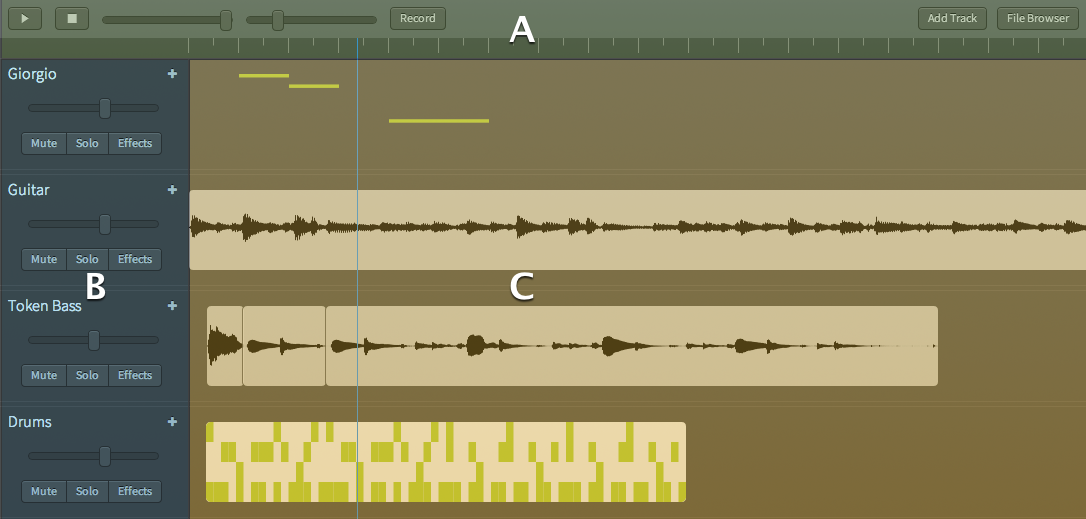
\includegraphics[width=\linewidth]{images/editor_overview_sections.png}}
    \caption[Editor Overview]{Editor Overview}
    \label{fig:editor-overview}
  \end{figure}

\end{landscape}
\newpage

\section{Structure}
\label{concept-overview}

The editor's structure is derived from Garageband, a DAW that is developed by Apple and which is part of their iLife software package\footnote{\url{http://www.apple.com/mac/garageband/}, last checked on 25/03/2014}. Garageband has a clear and easy to use user interface which is designed for both novice an expert users. The initial interface (\reffigure{fig:garageband-screenshot}) is simple and does not provide too many options. It can however be individualized by the user so that it fits the user's need and mental model. These options do not exist in the prototype of this thesis's editor, it just uses the same layout that is used in Garageband as well. The color palette for the editor's design is mainly inspired from Logic Pro X\footnote{\url{https://www.apple.com/logic-pro/}, last checked on 25/03/2014} (see \reffigure{fig:logic-screenshot}) and was built with the help of Adobe's Topcoat CSS package (\url{http://topcoat.io/}, last checked on 24/03/2014). Although the main structure was taken from Garageband, most other DAWs have a similar structure and it is easy for users to understand other DAWs, once they have become familiar with the concept of one of them (see \refchapter{ch:daw-apps}). 

The editor's user interface is split into three different parts (see \reffigure{fig:editor-overview}). Part A is the global control interface. The buttons on the left control the global playback of the arrangement. When the playback has been started, the blue line animates in the speed of the playback and acts as a progress indicator. It can also be controlled by clicking the vertical lines at the bottom of part A. A click on these lines causes the playback to jump to the selected position. The lines have different sizes to indicate time ranges. A longer line marks a second and a shorter line half a second. Next to the playback buttons are two range elements. The first one controls the master volume and the second one controls the zoom level. The zoom level influences the preview size of each of the arrangement's pieces. The button to the right of the range elements triggers the recording of the piece. Recording is only supported in real-time, so it works in the same way as tape recorders. When it is pressed, the playback starts, the button flashes red and the master output is recorded. The recording has to be stopped manually as well. After stopping the recording, the recorded file will be downloaded automatically. The button that says `Add Track' opens up a dialog that lets the user choose a type of track to add to the arrangement. The button that says `File Browser' opens up the file browser interface (see \refchapter{concept-import}).

Part B of the editor's layout contains the control panels for each of the tracks that were created by the user. Each track has an editable title, a volume control that only influences the current track's volume and it has buttons to turn on the mute or the solo mode of a track (see \refchapter{impl-tracks}). A third button `Effects' is also part of the control interface and it was designed to trigger an effects control panel for a track. Due to time limitations, this panel has not been implemented in the end. The `+' button in the upper right hand corner of the control panel adds a new piece to the track.

Part C shows previews for the individual pieces of the arrangement. The term pieces refers to audio pieces that have been created by using the editor's audio modules. Each track has a certain type and therefore only pieces of that type can be arranged in it. The different types of pieces and audio modules are explained in more detail in \refchapter{concept-modules}. The visual position of the previews determines their position in the arrangement and it can be changed by simply dragging them to the desired location. The properties of each piece can be changed by opening up their edit-interfaces that show up when they are double-clicked.

\section{Audio Modules}
\label{concept-modules}

Based on the capabilities of the Web Audio API (see \refchapter{ch:audio-theory}) and by looking at other DAW software, four different audio modules have been identified that build the foundation of a DAW. This chapter will show the prototypical web-based user interface for all four modules and it will explain their functionality.

\subsection{Recording}
\label{concept-recording}

\subsubsection{Preview}
\label{subsub:recording-preview}

The most basic element that needs to be in a DAW application is the recording functionality. It is essential that users can record and save audio signals e.g. from a microphone or a plugged in instrument like a guitar. The visual representation of a recording in all DAWs is the signal's waveform and therefore is also represented as a waveform in this editor as it can be seen in the `Guitar' and in the `Token Bass' track in \reffigure{fig:editor-overview}. It shows the amplitude alterations over time and indicates which part of a recording is louder than others. From that, the user can conclude which part of the recording is shown.

\subsubsection{Recording the signal}
\label{subsub:recording-ui}

\begin{figure}[htb]
  \centerline{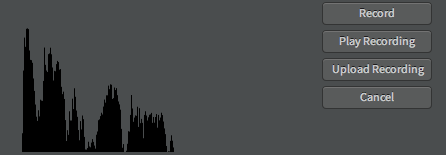
\includegraphics[width=\linewidth]{images/recording-a-signal.png}}
  \caption[Recording the signal]{Recording the signal}
  \label{fig:editor-recording-a-signal}
\end{figure}

\reffigure{fig:editor-recording-a-signal} shows the user interface for recording the user's input signal. The input could come from an external sound card, as well as from an internal microphone. The view is shown when the `+' button on a recording track is pressed. As soon as the user has agreed to give the application read access to the input signal, a visualization of the input signal is displayed that shows the frequency spectrum of the real-time data (see \refchapter{impl-recording-piece}). The user can initiate the recording by clicking the `Record' button which will flash red while recording. After finishing the recording, the `Play Recording' button plays the currently recorded bit and the `Upload Recording' button will upload the recorded file to the server and insert it into the current track.

\subsubsection{Editing a recording}
\label{subsub:recording-edit}

\begin{figure}[htb]
  \centerline{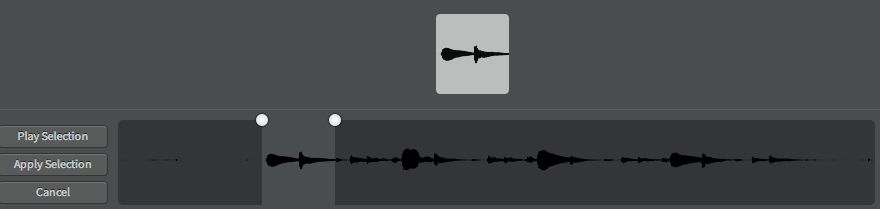
\includegraphics[width=\linewidth]{images/editing-a-recording.png}}
  \caption[Editing a recorded signal]{Editing a recorded signal}
  \label{fig:editor-editing-a-signal}
\end{figure}

In \reffigure{fig:editor-editing-a-signal} the edit interface for a recording is shown. Users have the ability to select a part from the recording which will then be used in the playback of the arrangement. In the example, only a small part from a longer recording is taken. This feature is especially useful to get rid of gaps from the start or the ending of a recording. A part is selected by dragging the two handles to the desired position of the recording. In order to check if the correct part has been selected, the user is able to playback the selection with the `Play Selection' button.

\subsection{Drum Machine}
\label{concept-drum}

\subsubsection{Preview}
\label{concept-drum-preview}

The drum machine preview can be seen in the track `Drum' in \reffigure{fig:editor-overview}. Each green rectangle stands for a beat in a pattern. The white parts are beats in a pattern that are not played. This kind of visualization is common in all DAW application (see \reffigure{fig:logic-screenshot} and \reffigure{fig:ableton-screenshot}). The width of the rectangles is defined by the amount of beats in a pattern and the zoom level of the editor. The height depends on the amount of different instruments in the specific drum kit.

\subsubsection{Editing}

\begin{figure}[htb]
  \centerline{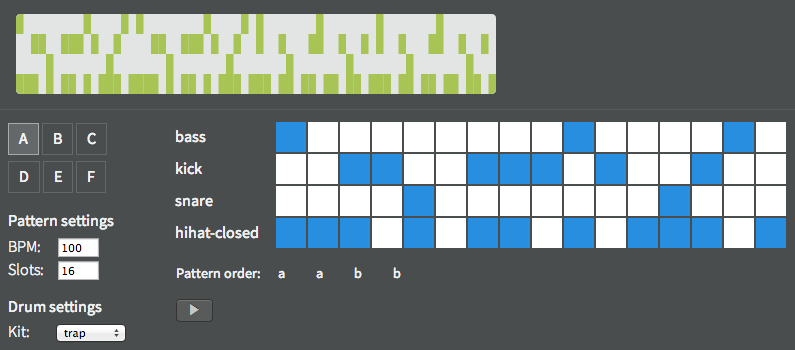
\includegraphics[width=\linewidth]{images/drum-edit.png}}
  \caption[Editing a drum loop]{Editing a drum loop}
  \label{fig:editor-editing-a-loop}
\end{figure}

\reffigure{fig:editor-editing-a-loop} shows the editing view for a drum machine piece. The grid to the right is used to activate and deactivate beats for the specific instruments. A blue rectangle means that the instrument will be played when this beat is being played and a white rectangle indicates a pause. The captions on the left of the grid represent the individual instruments. Again, this kind of user interface is very common among other DAWs as well and this one in particular is derived from FL Studio's\footnote{\url{http://www.image-line.com/flstudio/}. last checked on 25/04/2014} step sequencer (see \reffigure{fig:flstudio-screenshot}). The list of letters to the left stands for the amount of different patterns that can be created for a single drum machine piece. The order of patterns can be changed in the `Pattern Order' list by dragging patterns onto it and by using the order-arrows (only visible when hovered). This feature allows users to create complex pattern schemes in only one piece. A not so common feature that is supported in this editor is that for each pattern, a different speed (`BPM') and slot setting can be saved. This comes in handy when a complex pattern order needs a fill-in or a pause. The `Kit' select element gives the user the opportunity to change the drum kit, and therefore the sound for each beat. To the right there is also a play button which can be used to preview the drum pattern while editing it. The currently playing beat will be highlighted during the playback.

\subsection{Synthesizer}
\label{concept-synth}

\subsubsection{Preview}
\label{concept-synth-preview}

The preview of the synthesizer shows the individual tones and their length in a small version so that users can roughly see which tone will be played at which time. The vertical position of each tone is defined by its pitch (lower pitch - higher position) and its width is defined by the tone's length without an eventual release. It can be seen in the `Giorgio' track of \reffigure{fig:editor-overview}.

\subsubsection{Synthesizer Settings}
\label{concept-synth-settings}

\begin{figure}[htb]
  \centerline{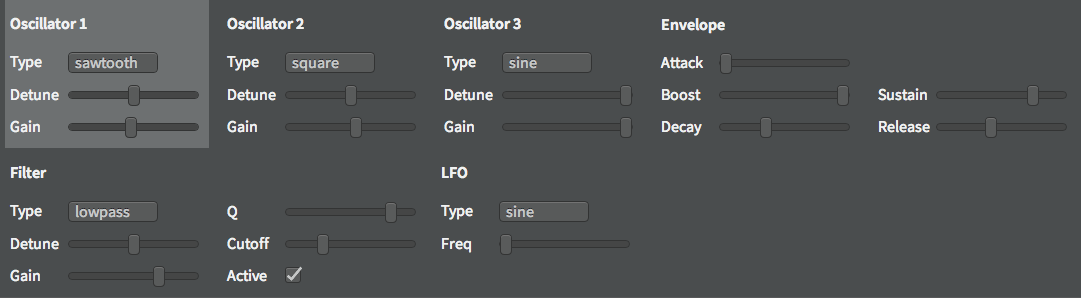
\includegraphics[width=\linewidth]{images/synth-settings.png}}
  \caption[The synthesizer's settings]{The synthesizer's settings}
  \label{fig:editor-concept-synth-settings}
\end{figure}

The synthesizer settings reveal that the synthesizer is a polyphonic synthesizer that features three individual oscillators for the sound generation. For each oscillator (`Oscillator 1-3'), the type of wave, the detune settings and the gain can be set. Detune is used to detune the pitch of the oscillator so that a more rich sound can be created. The detune settings allow an oscillator to be pitched an octave up and down. In the envelope settings, all classic parameters of an ADSR envelope can be defined (see \refchapter{sec:adsr-envelope}). The boost parameter is used to define the peak volume before the decay kicks in. The `Filter' form lets users choose and fine-tune a filter that will be used to shape the sound of the three oscillators. It can be toggled by ticking the `Active' checkbox. In the `LFO' section, an LFO (see \refchapter{sec:webaudio-synth}) can be activated and set to the desired sound. All sections will be highlighted when they are hovered so that the user always knows which parameters belong to which module of the synthesizer.

\subsubsection{Notes Grid}
\label{concept-synth-grid}

\begin{figure}[htb]
  \centerline{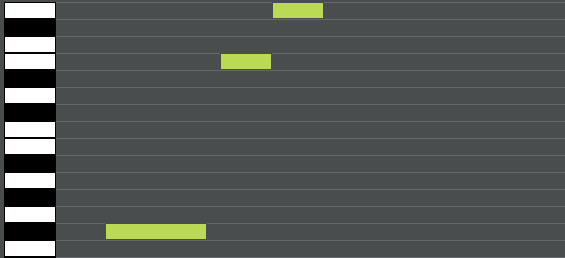
\includegraphics[width=\linewidth]{images/notes-grid.png}}
  \caption[The notes grid]{The notes grid}
  \label{fig:editor-concept-notes-grid}
\end{figure}

The notes for a synthesizer piece can be edited from the user interface that is shown in \reffigure{fig:editor-concept-notes-grid}. Similarly to the beats grid of the drum machine piece, the notes grid shows the notes on the right side. Each note can be dragged around to change its position in time and it can be deleted by double clicking it. A note is added to the grid by double clicking a note line. Its length can be changed by dragging its right edge. On the left, all notes of the keyboard are shown. Users are able to preview a note by playing it on the computer keyboard. The corresponding note will be played back and then highlighted in the user interface. The playback of all notes can be triggered using a play button at the bottom.

\subsection{Import \& File Browser}
\label{concept-import}

\begin{figure}[htb]
  \centerline{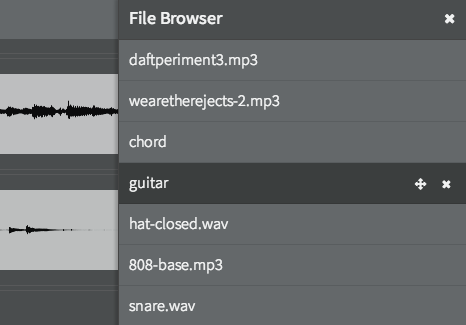
\includegraphics[width=.68\linewidth]{images/file-browser.png}}
  \caption[The file browser]{The file browser}
  \label{fig:editor-concept-file-browser}
\end{figure}

The fourth essential audio module that is present in every DAW is the ability to upload arbitrary sound files and use them in an arrangement. The editor supports this as well and audio files can be uploaded by dragging them onto recording tracks. They will be uploaded to the server automatically and then added to the file browser which can be seen in \reffigure{fig:editor-concept-file-browser}. All recordings and uploaded files will be listed there. In the figure, the `guitar' file is selected. The name can be edited in place and the file can be added to tracks by dragging it at the drag handle. It can also be deleted by using the `delete' button to the right.

\section{Synchronization}
\label{concept-synchronization}

All operations on pieces will be synchronized between all participating clients in real-time. The algorithm that realizes the synchronization has been described in \refchapter{ch:sync-theory} and its implementation will be described in \refchapter{impl-sync-algorithm}. The visual impact of the synchronization is minimal. Since the synchronization should happen in real-time without user interaction, the remote changes can be applied to the pieces and their edit interfaces while the editor is in use. If for example, the position of a piece is changed because user A dragged the piece to another position, the piece will also jump to this position in user B's editor. Also, all previews and edit-interfaces will be updated accordingly in real-time (e.g. the beats grid), so that even when two users are editing the same piece, the other user's changes can be taken into account and users can truly work on all pieces collaboratively. However, changes will only be applied when operations are finished and no in-between states are synced between the clients. For example, when a user edits the title of a track. The change of the title will only be sent to the server once the user has finished editing the title. The same applies to position changes of pieces. The position of the piece while dragging it will not be synchronized until the user has released the dragged element. In-between states are not synced because they can distract the other users while they are editing other parts of the arrangement.

\part{\ Implementation}
\label{part:implementation}

\chapter{Editor}
\label{ch:impl-editor}

%!TEX root = ../../thesis.tex
\section{Overview}

The application that was described in \refchapter{part-concept} was implemented mostly as a single-page JavaScript application with a JavaScript backend. The following chapters will describe the technologies that were used to implement the frontend editor. Furthermore, it will show in detail how the most important components and the custom techniques of the editor were developed.
%!TEX root = ../../thesis.tex
\section{Technology}

\subsection{AngularJS}
\label{subsec:technology-angular}

The core of the frontend editor is based on the JavaScript framework AngularJS\footnote{\url{http://angularjs.org/}, last checked on 20/03/2014}. It provides useful abstractions and concepts to organize JavaScript applications. The next chapters will contain details about how the editor's components were developed with the help of AngularJS components, so it is important to mention the core principles of the framework briefly.

AngularJS is built on top of the two concepts ``separation of concerns'' and ``dependency injection''. Separation of concerns describes that applications should be built from small, separated modules \cite[p. 8]{lerner2013ngbook}. AngularJS provides several base modules from which developers can create their own modules, which then form their application. Some of these modules are `directives' and `controllers' and they are the modules that were mostly used to create the audio editor.

\textbf{Directives} are modules that either create completely new HTML elements with custom layout and functionality, or they can be used to add custom functionality to already existing HTML elements\footnote{\cite[p. 61ff]{lerner2013ngbook}}. If written in a granular way, directives can be reused in many places of an application, so that common functionality does not need to be rewritten. An example for a reused directive in the audio editor is the \code{draggableDirective}, which adds drag and drop functionality to existing HTML elements. The functionality of these elements is described in more detail in \refchapter{impl-recording-piece}. As a rule of thumb, directives should be used whenever there is the need for accessing DOM elements and their events.

\textbf{Controllers} are used to add logic to HTML templates or to directives\footnote{\cite[p. 25ff]{lerner2013ngbook}}. AngularJS comes with its own template engine that supports declarative definitions and declarative two-way bindings. It is best to show the connection of controllers and templates in a short example:

\begin{lstlisting}[language=HTML, caption=A simple AngularJS template, label=lst:angular-template]
  <div ng-controller="MyController">
    <input ng-model="test" />
    <button ng-click="showValue()">Show</button>
  </div>
\end{lstlisting}

The template shown in \reflisting{lst:angular-template} declares that its functionality should be served from a controller called \code{MyController} (line 1). Its HTML input element should be bound to the value of a model called \code{test} (line 2) and a method called \code{showValue} should be called when the button in line 3 is clicked. All the attributes in this example that start with \code{ng-*} are directives that are part of Angular's core.

\begin{lstlisting}[language=JavaScript, caption=A simple AngularJS controller, label=lst:angular-controller]
  app.controller("MyController", ["$rootScope", "$scope",
    function($rootScope, $scope){
      $scope.test = "Timah";

      $scope.showValue = function(){
        alert($scope.test);
      };
  }]);
\end{lstlisting}

The context for the referenced model \code{test} in line 2 and the method \code{showValue} is provided by a \textbf{scope} which comes with the controller that is defined in \reflisting{lst:angular-controller}. A scope is used for keeping the application's data and for referencing methods in HTML templates. Furthermore, scopes can also be used to emit and listen to events, similar to DOM events. AngularJS defines which controller to instantiate by looking at the name that is provided from controllers (line 1). The value for the input element from \reflisting{lst:angular-template} comes from the variable that is assigned to the \code{\$scope} in line 3. Its value is bound to the template in two-ways. First, it will always be updated in the template, when \code{\$scope.test} changes in the program's logic. Secondly, whenever the value of the input element is changed by a user, \code{\$scope.test} is updated accordingly. The method that was referenced in the button from the above template is also added to the \code{\$scope} (line 5) and each time the button is pressed, the current value of \code{\$scope.test} will be alerted.

Another AngularJS core principle is demonstrated in \reflisting{lst:angular-controller}: Dependency Injection (DI). The controller itself is a simple JavaScript function that expects the two parameters \code{\$scope} and \code{\$rootScope}. Both parameters are included via dependency injection, a flexible way to define dependencies of a function. The module that resolves dependencies from the name of the parameter and injects them into the functions (the so-called \code{injector}), is capable of dynamically changing dependencies at runtime, which is the perfect setup for mocking dependencies when testing. DI therefore prevents that dependencies are loaded from a global namespace, which makes testing of components very hard\footnote{\cite[p. 149ff]{lerner2013ngbook}}.


\subsection{Grunt}
\label{subsec:technology-grunt}
Since AngularJS embraces a modular architecture, the frontend application is split up into many files and folders and an initial load of all files individually would slow down the application startup immensely. Therefore, an application compiler is used to concatenate all files into only four different files. The compile task is implemented as a Grunt\footnote{\url{http://gruntjs.com/}, last checked on 21/03/2014} task. Grunt is a build tool which is written in JavaScript and which provides many modules that help organizing and compiling frontend applications. In addition to simply concatenating the application, Grunt is also used to minify the application code before it is deployed to a server, in order to have an even faster load time. As mentioned before, the application is split up into only four files in the end. The main application logic, meaning all self-written AngularJS directives, controllers and other components, reside in the `app.js' file. All templates are added to `templates.js' and all external libraries, like AngularJS, are put into `vendor.js'.

\subsection{Stylus}
\label{subsec:technology-stylus}
The fourth file is `app.css', which is the compiled version of all Stylus\footnote{\url{http://learnboost.github.io/stylus/}, last checked on 21/03/2014} files. Stylus is a CSS pre-processor which provides a cleaner syntax, many helper functions and variables, e.g., for writing prefix-free\footnote{New and experimental CSS features are often introduced with so-called vendor prefixes e.g. \code{-webkit-featureName} until browser vendors are convinced they are stable enough and they fulfill the CSS specification.} CSS or for calculating colors and sizes in relation to other CSS definitions.
%!TEX root = ../../thesis.tex
\section{Arrangement}

The arrangement is the top-level data structure that contains the metadata of a project and all tracks and pieces. All data is organized into one single JSON object so that it is easier to create and apply diffs in the synchronization module (see \refchapter{impl-sync-algorithm}). Also, it is much easier to save single documents without cross-references in CouchDB (see \refchapter{backend-technology-couchdb}). Regardless, the data structure is simple and does not need to be normalized into different entities because no object in an arrangement will ever be referenced from other arrangement objects.

\begin{lstlisting}[language=JavaScript, caption=An arrangement's data structure, label=lst:arrangement-structure]
{
  id: "arrangement_id",
  title: "Never gonna give you up",
  owner: "user_id",
  participants: ["user_id"],
  tracks: [ Object ],
  buffers: [ Object ]
}
\end{lstlisting}

\reflisting{lst:arrangement-structure} shows that the most important information about arrangements is kept in the \code{tracks} array (line 6, see \refchapter{impl-tracks}) and the remaining information is mainly used in the backend to check if users are allowed to edit the document (\code{owner} and \code{participants}, line 4f) or to have an overview over all uploaded buffers (\code{buffers}, line 7).

The frontend representation of the arrangement, however, is an important node in the editor's node graph (see \refchapter{impl-node-graph}) and provides the master audio node that connects all available audio nodes to the speakers. Additionally, it manages almost all data structure operations such as adding and removing tracks or pieces. It handles the initialization of the synchronization module and takes care of applying the changes that are received from the server. The scheduling module (see \refchapter{sec:impl-scheduling}) also relies on the arrangement because the arrangement is capable of determining the total length of the project and looks up soon-to-be scheduled pieces.

Another task of the arrangement object is to handle the upload of files and to add them to the list of buffers. Vice versa, it also provides helper functions to delete uploaded files and ensures that all the file's associated pieces are also deleted so that the data structure does not contain unresolvable audio files.
%!TEX root = ../../thesis.tex
\section{Tracks}
\label{impl-tracks}

A track is the data structure that represents a row of pieces as shown in \refchapter{concept-overview}.

\begin{lstlisting}[language=JavaScript, caption=A track's data structure, label=lst:track-structure]
  {
    "id": "track_id",
    "title": "Guitar",
    "type": "recording/drums/synth",
    "gain": 0.9,
    "pieces": [ Object ]
  }
\end{lstlisting}

Its data structure contains information about the track's \code{gain} (line 5, \reflisting{lst:track-structure}), all its associated \code{pieces} (line 6) and its \code{title} (line 3), which makes it distinguishable from other tracks. The most important attribute is its \code{type} (line 4), because it influences the track's function and behavior. 

The editor prototype supports three different types: `recording', `drums' and `synth'. Each of these types makes the frontend's track object behave differently. The `recording' type adds drag and drop support for audio files which means that users can drag audio files from their computer onto a `recording' track and the file will be uploaded to the server and added to the track at the position it was dropped onto. When a file is dragged over a track, the track object checks if the file type is supported and provides visual feedback if the file type is not supported (e.g. for text files). In addition to local files, the track object also supports dragged buffers from the file browser (see \refchapter{concept-import}). This feature makes use of the native drag and drop API of HTML5 which adds events like `drag' and `dragover' to normal DOM elements and provides access to the \code{File} objects that are dragged from the local computer onto the website \cite{bidelman2010dnd}. Additionally, the API can make every HTML element draggable by adding a `draggable'\footnote{\cite[chapter: Creating draggable content]{bidelman2010dnd}} attribute to it. When a user starts dragging such an element, the above mentioned events will also fire for normal HTML elements. In case of dragged HTML elements, the API does not provide access to a \code{File} object but allows to add data to the event via its \code{dataTransfer} property\footnote{\cite[chapter: The DataTransfer object]{bidelman2010dnd}}. If, for example, a buffer is dragged from the editor's file browser, the associated buffer's \code{id} is added so that the track object is able to determine the type of the dragged object.

Additionally, the \code{type} parameter influences the functionality of a track's `add' button. Depending on the \code{type}, a new piece is added to the current track.

Another role of the track object is to handle the `solo' and `mute' states. The `solo' state mutes all other tracks, so that only this track can be heard when playback is started. The `mute' state mutes this track so that it is not heard in the playback. Both state changes are propagated as events from AngularJS's \code{\$rootScope} so that tracks can react to the state changes of other tracks e.g. turn down their volume when another track's `solo' mode is activated. A track's volume is controlled by two independently acting \code{GainNodes} (see \refchapter{impl-node-graph}) and its `solo' and `mute' state are not synchronized across the clients (see \refchapter{sub:sync-tracked-values}).
%!TEX root = ../../thesis.tex
\section{Recording Piece}
\label{impl-recording-piece}

The recording piece is a data structure that represents the user's recordings and uploaded audio files that can be used in `recording' tracks.

\begin{lstlisting}[language=JavaScript, caption=The recording piece's data structure, label=lst:recording-piece]
{
  "buffer_id": "buffer_id",
  "position": 7.32,
  "offsetStart": 2.04,
  "offsetEnd": 1.51,
  "id": "piece_id"
}
\end{lstlisting}

Its data structure is the simplest of all pieces because it basically only needs a reference to its buffer file (line 2, \reflisting{lst:recording-piece}) and the associated position at which it should be played (line 3). In addition to that, some recording pieces also contain information about offsets from the start and from the end (line 4f) which should be skipped in the playback.

The visual representation of a recording piece is the waveform of its associated audio file (see \refchapter{concept-recording}). A waveform is created by reading out the buffer's PCM audio data and rendering those values onto a \code{canvas} element. PCM stands for pulse-code modulation and it is a standardized way to represent a sampled audio signal. It stores the audio signal's amplitude for each sample that was taken in values of ranges from -1 to +1. A typical sample frequency for audio signals is 44.1kHz \cite[p. 26]{park2009introductionto}. The rendering algorithm takes the editor's current zoom level (see \refchapter{concept-overview}) into account and averages the sampled regions into one pixel wide chunks.

\begin{lstlisting}[language=JavaScript, caption=Simplified waveform algorithm, label=lst:waveform]
  var width = buffer.duration * pixelsPerSecond;
  var channelData = buffer.getChannelData(0);
  var length = channelData.length;
  var stepSize = Math.ceil(length / width);

  for(var i = 0; i < width; i++){
    var min = Math.min(i, stepSize, channelData);
    var max = Math.max(i, stepSize, channelData);

    rect(i, (1 + min) * middle, 1, (max - min) * middle);
  }
\end{lstlisting}

The waveform's width in pixels is defined by the product of the buffer's \code{duration} and the editor's zoom level in relation to pixels (line 1, \reflisting{lst:waveform}). The PCM data can simply be read from the buffer by calling its \code{getChannelData} method (line 2). It is important to average the PCM data because it is needed to correctly transform the PCM data into the editor's time space. The width of the rendered element is much smaller than there are entries in the data array because of the high sampling frequency. It is not a classical average calculation but a search for the minimum and maximum value of a certain part in the data (line 7f), because an average does not represent the shape of the signal's wave correctly and could be nulled from oscillation in the audio signal. So each pixel of the canvas element in the end represents the min and max of several hundred samples from the original data. Those values are rendered as a 1px wide rectangle which is vertically centered on the canvas (line 10).

Just like all other pieces, the recording piece's position can be changed by dragging it to the desired position in the track. Instead of using the previously described HTML5 drag and drop API (see \refchapter{impl-tracks}), pieces use a self-written drag and drop module because when using the native API for moving the original element, the events stopped firing after some time, which rendered this solution useless.

The self-written module uses standard DOM events to emulate the behavior of the native module. It starts by detecting a `mousedown' event on one of the draggable DOM nodes. A node is activated by simply adding a special attribute to it. This attribute is detected by AngularJS, which will then trigger a custom directive that adds the drag and drop functionality. After the `mousedown' event has been detected, a handler which tracks the global mouse movement is attached to the document. For each `mousemove' event, a move-delta is calculated from the previous mouse position and then propagated as a `drag' event. In addition to the `drag' event, the module also propagates `drag-start' and `drag-end' events similarly to the native API. Based on this module, an abstract \code{draggablePiece} directive was created which is used to add drag and drop functionality to all pieces.

The module is also used for the implementation of the recording piece's edit view which allows the user to define offsets for the current piece. The handles for both offsets (see \refchapter{subsub:recording-edit}) inherit the base module's functionality and build their own functionality on top of the module's events. The recording edit view is another user interface that has to translate between visual representation and time representation. An offset's visual representation is a \code{div} element whose width can be changed by dragging one of the handles. Once the handle is released, the module needs to calculate the actual time representation of the \code{div's} width. In both cases, the width of the element needs to be divided by the current value of \code{pixelsPerSecond} (the editor's zoom level) to get the correct time representation.

Another important aspect of the edit view is that its state is not synchronized on all clients and a synchronization will only happen when the user applies the currently selected range for the recording. Otherwise, users would be able to remotely drag the handles from other users interfaces and the accuracy of the user interface could not be guaranteed. A more detailed description on which attributes are synced between clients and which are not, can be found in \refchapter{sub:sync-tracked-values}.


The third view that is related to the recording piece is the recording view (see \refchapter{subsub:recording-ui}). At its core, the recording view is based on an a new web API called \code{getUserMedia}. It gives access to the streams of the client's microphone, the client's camera and, in very recent releases, also access to a stream of the clients screen. The audio stream is of the highest interest for the editor, because it can be used as a Web Audio node and therefore for visualizations and recordings. As soon as the user has granted access to its microphone stream\footnote{Technically, the API is not limited to just give access to the user's microphone. It is capable of providing an auio stream from any of the user's audio input devices (microphone, line-in etc.).}, a real-time frequency spectrum of the audio signal is shown. The spectrum can be used to fine-tune the incoming signal, e.g. by changing an instrument's settings, a microphone's settings or by getting closer to the microphone. The algorithm for drawing the frequency spectrum is similar to the one shown in \reflisting{lst:waveform}, but instead of selecting the signal's \code{channelData}, its \code{frequencyData} is used to draw on the \code{canvas}.

It is important to understand that a signal's frequency data and it's channel data are two completely different representations. The channel data is a representation in the time-domain, meaning it shows the signal's data in relation to time. When drawn onto a canvas, the x-axis is measured in time values\footnote{\cite[p. 40f]{park2009introductionto}}. A signal's frequency data, however, is the representation of a signal in the frequency-domain and a plotted version of the data will have an x-axis measured in frequencies\footnote{\cite[p. 276f]{park2009introductionto}}. The conversion of the signal from one to the other domain is done with the help of a Fourier Transformation. The Fourier Transformation is capable of extracting frequency data from a time-domain sample and of transforming frequency-domain data into time-domain data \cite{riffle2011fourier}. The transformation of a signal is a very CPU-intensive operation and is therefore not executed in JavaScript. All implementations of the Web Audio API come with a C++ implementation of the Fast Fourier Transformation\footnote{Fast Fourier Transformation is an algorithm to calculate the fourier transformation of a signal. \cite[p. 319f]{park2009introductionto}} and only the computed results of the transformation are made available through the API \cite[chapter: 7.6.5]{wilson2014webaudiospec}.

The recording functionality of the recording view comes from the Recorder.js library\footnote{\url{https://github.com/mattdiamond/Recorderjs}, Matt Diamond, last checked on 20/03/2014}, a de-facto standard library which records the output of Web Audio nodes. For that purpose, it uses another relatively new Web API called \code{WebWorkers}. They allow to execute JavaScript code in parallel to the main user interface thread. This functionality is needed because the \code{Recorder} takes the raw quantized audio signal and transforms it into reusable \code{Buffer} objects or \code{WAV}\footnote{WAV is a file format which is commonly used to encode audio data.} files, which is a CPU-intensive operation. After finishing the recording, the computed \code{WAV} file is uploaded to the server and then added to the list of available files.
%!TEX root = ../../thesis.tex
\section{Drum Machine}
\label{impl-drum-machine}

\begin{lstlisting}[language=JavaScript, caption=A drum machine's data structure, label=lst:drum-structure]
  {
    "type": "drum",
    "position": 0.78,
    "drumType": "808",
    "patternOrder": ["a","b"],
    "patterns": { a: Object, b: Object (...) }
  }
\end{lstlisting}

A drum machine piece is made of a meta data structure (\reflisting{lst:drum-structure}), which contains information about pattern order (line 5) and the drum kit type (line 4), and it also contains the information of all patterns (line 6).

\begin{lstlisting}[language=JavaScript, caption=A pattern's data structure, label=lst:pattern-structure]
  {
    "bpm": 70,
    "slots": 8,
    "beats": {
      "bass":  [1,0,0,0,0,0,0,0],
      "snare": [0,0,0,0,1,0,0,0]
      (...)
    }
  }
\end{lstlisting}

Patterns are the core data structure (\reflisting{lst:pattern-structure}) that contain the information about playback speed (line 2) and the beat order (line 5f). A value of \code{1} in one of the beat arrays means, that a beat will be played at this index. For example, the \code{snare} will only be played it index 5 (line 6). The \code{slots} property defines the length of the beat arrays. When the values is changed by the user, the arrays will either get cut off from the end (\code{slot} has been reduced) or they will be filled up with zeros (\code{slot} has grown).

Patterns have been specifically designed to allow musicians to be as flexible as possible. One drum machine piece can contain six different patterns (a-f). These patterns will all have the same base drum kit. Each pattern can have a different speed and a different amount of slots. The playback order for the patterns of a drum machine is defined in the \code{patternOrder} property. The example in \reflisting{lst:drum-structure} has an order of \code{["a", "b"]}. So pattern \code{a} is the first pattern to be played and \code{b} will be played afterwards. In this way, a wide variety of complex drum patterns and rhythms can be achieved by using only a single drum machine piece.

The preview playback (as seen in \refchapter{fig:editor-editing-a-loop}) uses a simple algorithm to loop the pattern. It is based on a high-frequency \code{Ticker}, an object that ticks another function every 30ms.

\begin{lstlisting}[language=JavaScript, caption=A pattern's loop algorithm, label=lst:pattern-loop]
  if(shouldPlayNextBeat()){
    beat = beat + 1;
    if(beat >= slots) beat = 0;

    nextBeatTime += secondsBetweenBeats();

    for(instrument in instruments){
      if(beats[instrument][beat]){
        play(instrument, nextBeatTime);
      }
    }
  }
\end{lstlisting}

For each tick, the algorithm first checks if a new beat should be played (line 1, \reflisting{lst:pattern-loop}). The method simply checks if the current time and the calculated time for the next beat overlap. Next, the current \code{beat} needs to be increased (line 2) and if the \code{beat} is the same size as the \code{slot} property, which defines the length of a pattern, it is reset to \code{0} so that the pattern starts over when its end has been reached (line 3). The exact time for the next beat is calculated by adding the amount of seconds per beat to the last time a beat has been played (line 5). The amount of seconds is calculated from the pattern's BPM. In the last step, the algorithm iterates over all instruments\footnote{Instruments here stand for the individual parts of a drum kit e.g. `hihat' or `snare drum'.} and checks if it should be played at the current beat\footnote{The current beat is the same as the beat index from line 5 of \reflisting{lst:pattern-structure}} (line 7ff). In the `global' playback, another scheduling algorithm is used for  performance reasons, which is explained in \refchapter{sec:impl-scheduling}.

There are several different drum machines from which users can choose. Each consisting of four to eight different instruments. So normally this would mean that for each drum kit that is used in an arrangement HTTP GET requests are started to load each instrument individually. In a case where an arrangement contains a lot of different drum kits, a lot of HTTP requests would be created which would slow down the application start. Thus, another technique is used to load drum kits: Audio sprites.

\begin{figure}[htb]
  \centerline{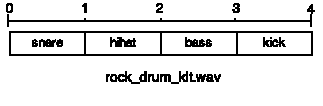
\includegraphics[width=0.9\linewidth]{images/drumkit_wav.pdf}}
  \caption[Audiosprites visualized]{Audiosprites visualized}
  \label{fig:audiosprites}
\end{figure}

The aim of audio sprites is to reduce the overall amount of HTTP requests, because they create an immense communication overhead. A benchmark\footnote{\url{http://janmonschke.com/Master-Thesis-Project/experiments/audio-sprites-benchmark/}, last checked on 21/03/2014} has shown\footnote{The test was executed from the same computer 10 times for each method in three different wirelesse networks. Caching was disabled while the tests ran.} that audio sprites reduce the load time by up to 50\% (see results in \refchapter{ch:speed-comparison}). Based on these results, all drum kits were implemented as audio sprites.

Audio sprites combine all individual audio files into one single large file. They also provide information about the position of the individual audio files into the one large file. As seen on \reffigure{fig:audiosprites}, the file \code{rock\_drum\_kit.wav} contains a \code{snare}, a \code{hihat}, a \code{bass} and a \code{kick} audio file. Each file is one second long\footnote{The real audio sprites leave some miliseconds pause between each individual file, so that there can be no overlapping audio data. For the sake of simplicity, these pauses are not shown in \reffigure{fig:audiosprites}}. The audio sprite for this drum kit would then contain the following offset information: \code{snare: [0, 1], hihat: [1, 2] (...)}. In the implementation, a drum kit is represented by one single buffer file (compare \refchapter{sec:webaudio-buffer}) and each time an instrument needs to be played, this buffer and the instrument's offset information are used to play the correct part of the drum kit's buffer (compare \refchapter{subsec:timing-in-web-audio}).
%!TEX root = ../../thesis.tex
\section{Synthesizer}
\label{impl-synth}

\begin{lstlisting}[language=JavaScript, caption=A synthesizer's data structure, label=lst:synth]
{
  "position": 1,
  "synthSettings": Object,
  "tones": [{
    "position": 0,
    "duration": 1,
    "note": "A2",
    "id": "tone_22"
  }]
}
\end{lstlisting}

The data structure of a synthesizer is the largest of all pieces because it contains the settings for each individual parameter of each synthesizer module (see \reffigure{fig:editor-concept-synth-settings}). All these settings are however omitted in \reflisting{lst:synth} because they would take up too much space. The \code{synthSettings} property (line 4) is basically a key-value description of the parameters. Each tone that should be played by the synthesizer is listed in the \code{tones} array. They consist of a \code{position} property (line 5), which describes the relative position of the tone in the current piece, a \code{duration}  property (line 6), which describes how long a tone is played, and the \code{note} property (line 7) which defines the pitch of the current note.

\medskip
\begin{figure}[htb]
  \centerline{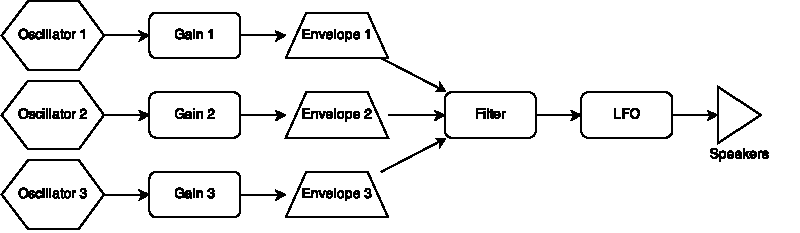
\includegraphics[width=\linewidth]{images/SynthesizerNodeGraph.pdf}}
  \caption[The synthesizer's node graph]{The synthesizer's node graph}
  \label{fig:synth-node-graph}
\end{figure}

The synthesizer that has been implemented for this editor is based on the early Moog synthesizer's design and its node graph is shown in \reffigure{fig:synth-node-graph}. It is a polyphonic synthesizer that uses three oscillators to generate the base sound. Each oscillator is routed through its own gain node which influences the volume of this specific oscillator and therefore it influences its impact in the mixed signal in the end. The gain node passes the signal on to an envelope which influences the oscillator's volume over time and from there it is passed to the filter. The filter shapes the sound of the mixed signal and passes it on to the Low Frequency Modulator which then influences the volume in an alternating manner. The LFO then passes the signal on to the speakers.

All modules haven been built from the base nodes which are supported by the Web Audio API and the envelope is based on the envelope which has already been sketched out in \refchapter{sec:adsr-envelope}. In order to play a tone, the tone's \code{note} property needs to be transferred into a base frequency which will then be the frequency that is used for each oscillator. The implementation of this translation is based on Stuart Memo's algorithm from his `QWERTY hancock' library\footnote{\url{http://stuartmemo.com/qwerty-hancock/}, last checked on 17/03/2014}.

One big challenge in implementing the synthesizer was that a manual garbage collection of unneeded oscillator nodes was needed because the amount of oscillator nodes grew fast over time and unused oscillators have a huge performance impact on the overall application. The algorithm for the garbage collection runs during the playback of the synthesizer piece and checks for unused and finished nodes at a specific interval which is based on a pre-calculated overall amount of needed nodes and the time that is between the tones.

The note grid's implementation, which was already shown in \refchapter{concept-synth-grid}, is based on the drag and drop elements that were already used in other pieces like the recording piece (see \refchapter{impl-recording-piece}). One tone in the grid consists of two draggable nodes. One that influences the relative position of the tone and one that influences the width, and therefore the duration, of the tone.
% %!TEX root = ../../thesis.tex
\section{Effects}
\label{sec:webaudio-effects}

\begin{quote}
  ``Anything more than three chords is just showing off.'' -
  Woody Guthrie
\end{quote}

In addition to filters (see \refchapter{sec:webaudio-filter}), there is a myriad of ways to shape sounds in order to create different effects. Two common techniques that can be used to create a variety of effects will be shown in this section: convolution and waveshaping.

\subsection{Convolution}

Convolution is most commonly used in audio programming for creating reverb effects. Reverb effects add the characteristics of locations to sounds. For example, by adding a reverb to the recording of a guitar chord, it can sound like it was recorded in a concert hall, a cave or under water. The base of this technique is the so-called Impulse Response (IR) which describes the characteristics of a system (here: the audio characteristics of a location) and its influence on an input signal \cite[p. 132ff]{park2009introductionto}. IRs are created by playing back a base audio signal (e.g. a clap) in a desired location. The playback is recorded and afterwards the original audio signal is deleted from the recording, so that only the room effect is left in the recording \cite[chapter: Room Effects]{smus2013webaudio}. In order to apply the IR to an arbitrary sound, the IR's signal is multiplied with the sound signal and the resulting signal contains the reverb effect. The mathematical model for this operation is convolution, which is why the effect is also often called convolution reverb\footnote{\cite[p. 139f]{park2009introductionto}}.

Convolution is a computationally intensive operation, thus it would result in a high CPU usage if done in JavaScript. The Web Audio API comes with a \code{ConvolverNode} \cite[chapter: ConvolverNode]{wilson2014webaudiospec}, which uses a C++ convolution engine under the hood to enable the computation in real-time\footnote{\url{https://chromium.googlesource.com/chromium/blink/+/32c15b00f4deb24f3f55156eba1c27fb506711d2/Source/modules/webaudio/ConvolverNode.cpp}, line 85, last checked on 19/03/2014}\footnote{Only Google Chrome's source is referenced here, but it is assumed that all other browser vendors also use a native engine for most Web Audio Nodes.}.

\begin{lstlisting}[language=JavaScript, caption=ConvolverNode usage, label=lst:convolver-node]
  var song = getSong("faith+1/01.mp3");
  var ir = getFile("reverb/church.wav");

  var convolver = context.createConvolver();
  convolver.buffer = ir;

  song.connect(convolver);
  convolver.connect(contxct.destination);
\end{lstlisting}

The above example (\reflisting{lst:convolver-node}) demonstrates the simple usage of the \code{ConvolverNode}. An IR is loaded from a file (line 2) and then assigned to the \code{buffer} of a newly created \code{ConvolverNode} (line 4f). Then, the \code{song} simply needs to be connected to the \code{convolver} (line 7) and the input signal is convolved with the IR's signal. The intense calculation is hidden and common Web Audio API patterns, like reusing buffers as IRs, are applied to make the \code{ConvolverNode} easy to use. In this case, the song playback would receive a hall effect similar to one that can be found in churches.

\subsection{Waveshaping}

Waveshaping is a technique to distort a sound signal. For this purpose, a shaping function is applied to an audio signal to shape the wave in a desired way \cite[p. 252]{curtis1996computer}.

\begin{figure}[htb]
  \centerline{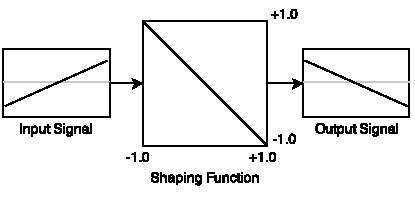
\includegraphics[width=0.75\linewidth]{images/waveshaping.pdf}}
  \caption[Using a waveshaping function to transform a signal -
  \protect\newline{\small based upon \cite[p. 255]{curtis1996computer}}]{Using a waveshaping function to transform a signal}
  \label{fig:waveshaping}
\end{figure}

The example in \reffigure{fig:waveshaping} shows a linear shaping function ($ f(x) = -x $) and a linear input signal. The output of the shaping function is an inverted input signal. For the purpose of simplicity, both, the input signal and the shaping function, are linear functions, but waveshaping is not limited to linear functions. In normal applications of waveshaping, the signal and the shaping function are non-linear. For faster computation, shape functions can be represented as in-memory look-up tables for values from -1 to 1. A typical application for waveshaping is the overdrive effect, which is well-known from the distorted sound of heavy guitar music.

In the Web Audio API there is a special node for waveshaping, the \code{Wave\allowbreak ShaperNode}. It uses a pre-stored wave function to shape the connected audio signal. The following example creates an overdrive effect and is taken from the \code{tuna} library\footnote{\url{https://github.com/Dinahmoe/tuna}, Dinahmoe, last checked on 20/03/2014}, which provides a variety of effects for the Web Audio API\footnote{For abbreviation, the part about loading and connecting a buffer, as seen in the examples before, is left out.}.

\begin{lstlisting}[language=JavaScript, caption=Using the WaveShaperNode, label=lst:waveshaper-node]
  var samples = 8192;
  var table = new Float32Array(samples);
  var amount = .7;
  var k = 2 * amount / (1 - amount),
      i, x;
  for(i = 0; i < samples; i++) {
    x = i * 2 / samples - 1;
    table[i] = (1 + k) * x / (1 + k * Math.abs(x));
  }

  waveshaper = context.createWaveShaper();
  waveshaper.curve = table;
\end{lstlisting}

For the representation of the curve, a \code{Float32Array} is used instead of a normal array (line 2, \reflisting{lst:waveshaper-node}), which is filled by iterating over the amount of \code{samples} (line 6) and calculating the function's value at the current point (line 8). In short, the above created curve table represents a variable version of the mathematical function $ f(x) = \frac{x}{abs(x)} $ which acts as a clipping function for the input signal. The clipping threshold is defined by the value of \code{amount} (line 3) and is typically a parameter that is defined by users.
%!TEX root = ../../thesis.tex
\section{Node Graph}
\label{impl-node-graph}

\begin{figure}[htb]
  \centerline{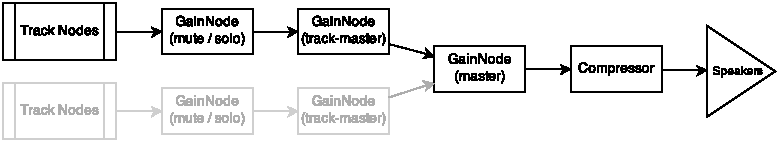
\includegraphics[width=\linewidth]{images/Node_Graph.pdf}}
  \caption[The editor's audio node graph]{The editor's audio node graph}
  \label{fig:nodegraph}
\end{figure}

\reffigure{fig:nodegraph} shows the editor's basic audio graph setup. Each track is wired in the same way. All individual audio nodes of a track (e.g. \code{BufferSourceNodes} in case of a recording track) are connected to their `mute / solo' \code{GainNode}. A \code{GainNode} is an audio node that controls the gain of all the nodes that are connected to it. The `mute / solo' \code{GainNode} controls a track's gain, when its `mute' or `solo' attribute changes. A muted track will have a gain value of \code{0} when its \code{mute} attribute is \code{true} and it will have a gain value of \code{1} if either its \code{mute} attribute or its \code{solo} attribute is \code{true}. All other tracks will have a \code{false solo} attribute if one of the tracks has a \code{true solo} attribute and their \code{gain} value will be \code{0}.

The `track-master' \code{GainNode} controls the overall gain value of the track, which is represented by a track's \code{gain} attribute. This attribute is synchronized and persisted across all clients. By separating the `track-master' from the `mute / solo' node, the editor has fine-grained control about the individual gain settings of the tracks and users can individualize their local track setup without interfering with other users' setups (e.g., if User A mutes track B and user C is currently working on track B's details, user C's track is not muted and he is still able to work on it).

Each track's `track-master' \code{GainNode} is connected to the editor's `master' \code{GainNode}. It controls the overall gain level. Its value is also not synchronized so that each user has full control over the playback's volume.

Before the editor's signal goes to the speakers, it is passed through a `compressor'. This node's purpose is to create a more homogeneous sound signal and to prevent the signal from being clipped because it is too loud. The Web Audio API already provides a node for this purpose, the \code{DynamicsCompressor Node}\footnote{\url{http://webaudio.github.io/web-audio-api/\#idl-def-DynamicsCompressorNode}, last checked on 21/03/2014}. It is also this node, which is used to record the arrangement (see \refchapter{impl-arrangement-recording}).

The node setup of all the different types of nodes is explained in detail in their individual implementation chapters. The `last' node in their setup always connects to the track's `mute / solo' node to pass its signal into the editor's node graph.
%!TEX root = ../../thesis.tex
\section{Scheduling}
\label{sec:impl-scheduling}

The scheduling system is a major backbone of any audio editing software. The playback of buffers and the timing of drum machines and synthesizers needs to be exact to the millisecond. Timing glitches cause unwanted effects on arrangements and can destroy the playback experience of a song. Inexact timing will also frustrate users because it is an error that renders the usage of the editor for song composition impossible.

As already described in \refchapter{subsec:timing-in-web-audio}, the Web Audio API provides an exact timing system. This system, however, does not provide a scheduler, it only comes with a way to exactly time individual Web Audio components and nodes (e.g. buffers and oscillators). All custom components (e.g. drum machines) need a custom timing component that builds on top of the provided timing methods. Not only do all custom components need their own timing mechanism but also the overall arrangement, which contains information on when to play which piece of a track.

A na\"ive approach to implement a scheduler for an arrangement would be to calculate the start time for all pieces and to start them all when the user initiates the playback. All individual nodes would then play at the precisely calculated time and the arrangement playback would be perfect. Nonetheless, this approach comes with some drawbacks.

Firstly, the scheduler would need to hold references to each node and its subnodes in memory in order to stop them when the user stops the playback of the arrangement. This also implies that all nodes would need to be created initially, which could, for a complex arrangement, take a non-trivial amount of time. Both issues also lead to a constant high usage of memory that might affect the performance of the editor.

Secondly, although it is not stated in the Web Audio specification\footnote{\cite{wilson2014webaudiospec}}, the initial very high amount of pre-scheduled audio events could have a negative impact on the audio playback and also the editor's performance. Scheduling each node upfront means that each individual sound of a drum machine would need to be scheduled upfront as well. This could, depending on the arrangement and used audio nodes, result in thousands of pre-scheduled nodes.

In order to have playback control over all these nodes, they would need to be kept in memory. The iteration over each individual node can take a non-trivial amount of CPU time which would block the main user interface thread. The editor's user interface needs to stay responsive and interactive the whole time. A negative scenario would be that the user interface would not react and freeze when the user wants to seek to a different position in the arrangement by clicking the position in the timeline element. All scheduled audio events would need to be stopped and restarted when seeking to a different point in the arrangement.

\subsection{Arrangement Scheduler}

For all the above mentioned reasons, a more complex scheduling system is needed that ensures that the following requirements are fulfilled:

\begin{enumerate}
  \item All sounds need to be timed precisely.
  \item The system needs to have a small memory footprint.
  \item The system does not block the main user interface.
\end{enumerate}

The main problem of the na\"ive scheduler was that it had to schedule and allocate all events at once, which led to many problems. Most of these problems can be overcome by introducing a gradual scheduler which schedules sounds depending on the current position in the playback of the arrangement. The basis for this scheduler is a combination of JavaScript's own timing methods (compare \refchapter{subsec:timing-in-js}) and the precise timing methods in the Web Audio API.

\begin{figure}[htb]
  \centerline{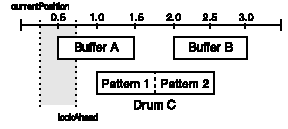
\includegraphics[width=0.9\linewidth]{images/Scheduler_Example.pdf}}
  \caption[Scheduler]{Scheduler}
  \label{fig:scheduler}
\end{figure}

\reffigure{fig:scheduler} shows an example arrangement with a Buffer that should be played at 0:00,5 minutes (Buffer A), another Buffer that should be played at 0:02 minutes and a drum machine, containing 2 patterns, which should start at 0:01 minutes.

The scheduler uses a \code{Ticker} object to gradually check if new pieces need to be scheduled. A \code{Ticker} uses JavaScript's \code{setInterval} to constantly notify listeners that a new interval has passed. So whenever an interval has passed, the scheduler scans the arrangement for unscheduled pieces using the following algorithm (\reflisting{lst:scheduling-pieces-p1}):

\begin{lstlisting}[language=JavaScript, caption=Detecting pieces that need to be scheduled, label=lst:scheduling-pieces-p1]
  for(piece in unscheduledPieces){
    var inLookahead = position < piece.position &&
                      position + lookAhead >= piece.position;

    var inBetween = position >= piece.position &&
                    position < piece.position + piece.length;
    (...)
  }
\end{lstlisting}

First, the scheduler checks if the current piece starts in the \code{lookAhead} window (line 2f). Therefore, the current \code{position} in the song, which is as well calculated in each interval, is compared to the piece's starting \code{position} and the \code{lookAhead} time frame. If the song \code{position} plus the \code{lookAhead} time is more or equal than the piece's \code{position}, the piece needs to be scheduled in this time frame. By using a \code{lookAhead} time comparison, the scheduler ensures that even in the case of a large delay in the \code{Ticker's} \code{setInterval}, all pieces will be scheduled correctly and none of them is skipped. Consequently, the \code{lookAhead} time is a multiple of the \code{Ticker's} interval time. The current implementation uses a \code{lookAhead} of three times the interval. The interval time itself is set to the shortest length of all pieces to ensure that no piece can be skipped by a interval that is too long and also to reduce the overall amount of timeouts, e.g. if a too short interval is chosen. In case of a song position of 0:01 minutes, only Buffer A would be scheduled initially.

This first check alone already ensures that the number of simultaneously scheduled pieces is reduced to the bare minimum. But it does not cover several edge cases and would also schedule all pieces that start before the current song position, even if the scheduler was started with a song position after their position in the song such as when the scheduler was started at 0:01,6 seconds and Buffer A would be scheduled as well, although it does not need to be scheduled.

The second check (line 5f) ensures to leave out pieces that ended before the scheduler was started by comparing the song \code{position} to the \code{piece's position} plus its \code{length}, which is the end time of the current piece. When the song's \code{position} is less than the end time of the piece and the song \code{position} is bigger than or equal to the \code{piece's position}, the scheduler sorts out ended pieces. In addition to that, the scheduler selects pieces that need to be scheduled with an offset. This case happens when the scheduler is started at a song position that lays between the beginning and the end of a piece, e.g. if the scheduler in \reffigure{fig:scheduler} would start with a song position of 0:01 minutes. Buffer A would need to be scheduled with an offset.

\begin{lstlisting}[language=JavaScript, caption=Scheduling pieces, label=lst:scheduling-pieces-p2]
  if(inLookahead || inBetween){
    var when = Math.max(piece.position - position, 0);

    var offset = Math.max(position - piece.position, 0);

    piece.start(when, offset);
    scheduledPieces.push(piece);
  }
\end{lstlisting}

If either the first or the second check was truthy, the piece will be scheduled (line 1, \reflisting{lst:scheduling-pieces-p2}). The exact point \code{when} to start the piece is calculated from the difference of the \code{song's position} and the \code{piece's position} (line 2). Also, in case the piece needs to be started with an offset, the offset is calculated by subtracting the \code{piece's position} from the current song \code{position} (line 4). In the last step, the piece is started and added to the list of scheduled pieces. The list of scheduled pieces is needed for the case that the user stops the playback of the arrangement and all scheduled pieces need to be stopped so that they do not play.

The described scheduling system does fulfill all three requirements. By using the \code{lookAhead} method it ensures that even if the system uses the inaccurate \code{setInterval} function, all pieces are scheduled precisely and also calculates offset positions. The overall memory footprint is very small because the system only keeps already scheduled top-level pieces (see \refchapter{subsec:local-scheduler}). Lastly, the system does not block the main user interface thread because cancelling pieces is very fast (due to the low amount of pieces) and the scheduling mechanism is triggered intelligently only when really needed.

\subsection{Local Scheduler}
\label{subsec:local-scheduler}

The intelligently selected interval of the above described scheduler solely reduces the computation time if only top-level pieces are handled. This works well for recorded pieces, but not so well for drum machine pieces or synthesizer pieces because the minimum interval time for these pieces would actually be much lower. These pieces are composed of many individual sounds with only a friction of a second delay in between them, which would lead to a lot more scheduling intervals and therefore to a much higher CPU usage. For this reason, these pieces have their own schedule-mechanism, which is triggered by the above shown arrangement scheduler. The arrangement scheduler is not aware of the fact that, for example, drum machine pieces are different from recorded pieces, because they share the same interface and can be triggered in the same way. They both have a \code{start} method (compare \reflisting{lst:scheduling-pieces-p2}, line 6) that accepts a point in time (\code{when}) and an \code{offset}. So the complexitiy behind the ``local scheduler'' is not exposed to the ``global scheduler'' (the arrangement scheduler).

\begin{figure}[htb]
  \centerline{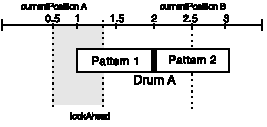
\includegraphics[width=0.9\linewidth]{images/Scheduler_Example_Drum.pdf}}
  \caption[Scheduler and sampler]{Scheduler and sampler}
  \label{fig:scheduler-sampler}
\end{figure}

All pieces that need an own scheduling mechanism are organised into patterns (see \refchapter{impl-drum-machine}), which themselves consist of the individual sounds and their timing information. These pieces use a sampler for their internal scheduling. \reffigure{fig:scheduler-sampler} shows an example of an arrangment with a drum machine (Drum A) that is composed of two patterns (Pattern 1 and Pattern 2). The global scheduler starts at 0:00,5 minutes and sees that Drum A needs to be scheduled to start in 0.5 seconds and calls the drum machine's \code{start} method. Behind the scenes it is not the drum machine's method but the drum machine's sampler's \code{start} method. The sampler also, just as the global scheduler, uses a \code{Ticker} object to gradually schedule notes or, more precisely, to gradually schedule patterns. One of the requirements for the scheduler is to have as few interval timeouts as possible to reduce the CPU usage. If the sampler were to schedule individual notes, the minimal interval time would be very low and would result in a lot of timeouts and extra calculation. Also, the offset error rate for small timeouts has a much bigger impact on the complexity of achieving an accurately timed playback than for bigger timeouts. For this reason, the sampler schedules whole patterns at once.

\begin{lstlisting}[language=JavaScript, caption=Scheduling patterns (sampler), label=lst:scheduling-patterns]
  if(this.hasNextPattern()){
    if((currentTime + lookAhead) > this.nextPatternTime()){
      this.scheduleNextPattern();
    }
  }else{
    cleanUpMemory();
  }
\end{lstlisting}

Similar to the global scheduler, the sampler uses a \code{lookAhead} time in order to determine if a pattern needs to be scheduled (line 2, \reflisting{lst:scheduling-patterns}). If a next pattern is detected and needs to be scheduled, all notes of that pattern are scheduled ahead (line 3). Otherwise, if there is no next pattern, the sampler can clean up the memory (line 6). This needs to be done, because references to all scheduled notes are kept in memory for the currently playing pattern to be able to stop them, when playback is stopped. Othwerwise, all scheduled drum notes would play even if the user has pressed the stop button. The calculation of the startup time for each note depends either on the drum machine's BPM or the position of the note in a synthesizer's arrangement.

In addition to pattern scheduling, the sampler also takes care of calculating the impact of offsets for each pattern. In \reffigure{fig:scheduler-sampler}, \code{currentPosition B} shows an example where a sampler needs to take an offset into its scheduling calculation. In this case, Drum A will be scheduled with an offset of 1.5 seconds which means that the sampler needs to schedule Pattern 2 and not Pattern 1. The sampler also needs to leave out all notes that were played before \code{currentPosition B}.

\begin{lstlisting}[language=JavaScript, caption=Calculating offsets (sampler), label=lst:scheduling-offsets]
  function(offset){
    forEachPatternInOrder(function(pattern, index){
      patternEnd += pattern.length;

      if(offset < patternEnd + pattern.length){
        currentPattern = pattern;
        return false;
      }else{
        patternEnd += pattern.length;
      }
    });

    var patternOffset = offset -
                (patternEnd - currentPattern.length);
    var beat = patternOffset /
                currentPattern.secondsBetweenBeats();

    beat = Math.floor(beat);
    currentPattern.beat = beat;
  }
\end{lstlisting}

The algorithm in \reflisting{lst:scheduling-offsets} is initialized with the \code{offset} that was determined from the global scheduler (line 1). As a first step, the algorithm detects the correct pattern from the pattern order that should be played at the current offset position (line 2ff). The current pattern lengths are summed up until the offset has been reached (line 5). After that, the relative offset of the current pattern is determined by subtracting the length until the current pattern (line 14) from the global \code{offset} has been reached, which results in the time that should be skipped for the current pattern. In case of the example in \reffigure{fig:scheduler-sampler} (\code{currentPosition 2}), the \code{patternOffset} should be 0.5 seconds. The step after that is different for the drum machine's sampler and the synthesizer's sampler but for reasons of simplicity, \reflisting{lst:scheduling-offsets} only shows the former implementation for note skipping. Through dividing the \code{patternOffset} by the current pattern's BPM (converted to seconds per beat), the algorithm is able to detect the amount of beats that need to be skipped (line 15f). This beat is then used as the base beat for the current pattern (line 19) and all beats before that will be skipped. The synthesizer's sampler uses a combination of all the above described techniques to determine the skipped notes and explaining it here would only repeat already covered implementation details.

The local scheduler ensures that all three requirements for an efficient scheduler are met. It adds a precises timing method for drum machines and synthesizers by pre-scheduling complete patterns. Although all played notes are held in memory for a short time, the \code{cleanUpMemory} method assures that unused notes are released to keep the memory footprint small. Lastly, the scheduling interval timeouts are kept to a minimum in order to reduce CPU usage.

%!TEX root = ../../thesis.tex
\section{Arrangement Recording}
\label{impl-arrangement-recording}

Arrangement recording is used to create a WAV file from the arrangement that can be played back in media players or uploaded to user profiles to music sharing websites. It uses the same library for recording which was also used in \refchapter{impl-recording-piece}.

The recording module hooks into its node graph directly in between the compressor and the speakers to buffer the audio signal (see \reffigure{fig:nodegraph}). The end of the recording is not triggered automatically and requires the user to press the recording button again, because the end of the arrangement cannot be calculated exactly. There might be a synthesizer piece at the end of a song with a high release time. The release time is not used in the calculation of a piece's length, thus an automatic recording stop could cut off a small fraction of the synthesizer's notes.

\chapter{Backend}
\label{ch:impl-backend}

%!TEX root = ../../thesis.tex
\section{Technology}
\label{backend-technology}

\subsection{NodeJS}
\label{backend-technology-nodejs}

The editor's server is written in NodeJS\footnote{\url{http://nodejs.org}, last checked on 25/03/2014} a server-side JavaScript platform. Through using JavaScript in the frontend and in the backend, the implementation of the synchronization algorithm (see \refchapter{impl-sync-algorithm}) was more easy because the same helper modules and, to some extend, even the same code could be used. There is good support for WebSockets in external NodeJS modules, which builds the foundation of the synchronization modules.

By default, NodeJS does not come with a dedicated web framework but only with core modules which are more low-level than other backend platforms such as Ruby on Rails\footnote{A ruby-based web framework, \url{http://rubyonrails.org/}, last checked on 24/03/2014} or Django\footnote{A python-based web framework, \url{https://www.djangoproject.com/}, last checked on 24/03/2014}. For this reason, Express\footnote{\url{http://expressjs.com/}, last checked on 24/03/2014} has been used to implement the backend. Express is a light-weight framework but it provides handy abstractions and building blocks to build complex web applications on top of it \cite[p. 176f]{cantelon2013node}.

\subsection{CouchDB}
\label{backend-technology-couchdb}

CouchDB\footnote{\url{http://couchdb.apache.org/}, last checked on 24/03/2014} has been chosen to be the database for the editor. It is a document-based no-SQL database, meaning that it stores data in documents rather than in rows and the data is not requested with SQL. The format of CouchDB documents is JSON, which makes it perfectly suitable for JavaScript backends and frontends. Instead of using SQL, data is queried using \code{views} on the data \cite[chapter: Finding Your Data with Views]{anderson2010couchdb}. \code{Views} consist of a \code{map} and a \code{reduce} function that are both used to pre-select and aggregate data for queries.

\subsection{Redis}
\label{backend-technology-redis}

Redis is an in-memory key-value database\footnote{\url{http://redis.io/}, last checked on 25/03/2014} which is used in addition to CouchDB. It is, however, not used to store project data or user data. Its sole purpose is to store user sessions. CouchDB has not been used for this purpose, because CouchDB and NodeJS might be run from two different servers and the request to create a session or to check if a session is valid would take much longer in this case. Since Redis is an in-memory store, all lookup- and write-operations are much faster.
%!TEX root = ../../thesis.tex
\section{Structure}

The backend implementation is based on a micro framework that has been developed on top of Express and bases itself loosely on the MVC pattern. It is a stateless framework and deals with HTTP connections for all requests that are not related to the synchronization module. The synchronization module uses WebSockets instead of HTTP.

\begin{figure}[htb]
  \centerline{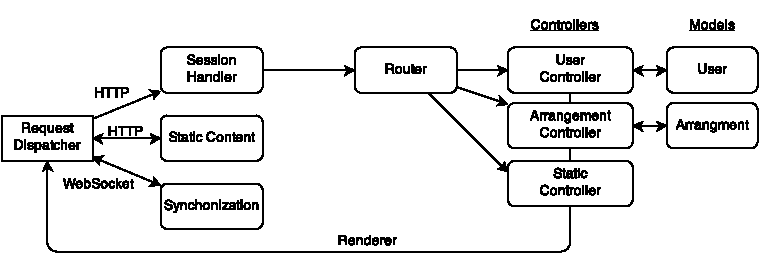
\includegraphics[width=\linewidth]{images/BackendDiagram.pdf}}
  \caption[The backend structure]{The backend structure}
  \label{fig:backend-structure}
\end{figure}

All requests are handled by the `Request Dispatcher' which, dependent on the URL and the type of the request (HTTP vs WebSocket), decides to which module the request will be forwarded. The simplest module is the `Static Content' module, because it simply loads all static files like the frontend JavaScript and the CSS from disk and delivers it to the client. It also takes care of delivering all uploaded audio files.

The synchronization module is initialized by WebSocket connections and it handles all sync-relevant operations which are explained in more detail in \refchapter{impl-sync-algorithm}.

Requests that are not handled by the two already mentioned modules are passed on to the `Session Handler' and the `Router'. The `Session Handler' ensures that all requests that reach the `Router' have a session attached to it so that they can be associated with a user. The `Router' basically consists of a `URL to Controller' lookup table and passes the request on to the `Controller' that is associated to the address of the current request. There are three main controllers. The `StaticSite' controller takes care of rendering the website's views into HTML. The `User' controller deals with sign-ups and rendering the user pages. The `Arrangement' controller creates and renders project files. All controllers have models associated that take care of the basic CRUD\footnote{Create Retrieve Update Delete} operations with the database.

The architecture of the framework has been developed in a modular way so that it can be reused for other websites as well. In order to implement a normal website that does not need the synchronization module, the module only needs to be removed and the framework can be used without it.

%!TEX root = ../../thesis.tex
\chapter{Synchronization}
\label{impl-sync-algorithm}
This chapter explains all details about both the frontend and backend implementation of  Differential Synchronization and the adoptions that were made during the development. 

As discussed in \refchapter{sec:realtime-discussion}, the implementation of the synchronization algorithm is based on WebSockets. The NodeJS module socket.io\footnote{\url{http://socket.io/}, Guillermo Rauch, last checked on 12/03/2014} is used as an abstraction layer on top of raw WebSockets because it adds support for rooms and sending messages in a request-response way, instead of plain one-way WebSocket messages. In addition to socket.io, jsondiffpatch\footnote{\url{https://github.com/benjamine/JsonDiffPatch}, Benjam\'{i}n Eidelman, last checked on 13/02/1014} is used as a key part of the implementation. It is used to create and apply diffs to the underlying JSON data structure on both sites.

\subsection{Protocol}
\label{subsec:ds-algo-protocol}

The synchronization is backed by an own protocol on top of WebSockets (see \refchapter{realtime-ws}), which is modeled after the control flow of the Differential Synchronization algorithm (explained in \reffigure{fig:DiffSync}). Further, the developed protocol adds a new message to the original control flow to make the synchronization more instant.

\begin{figure}[htb]
  \centerline{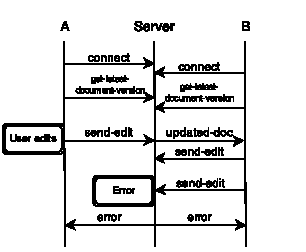
\includegraphics[width=0.8\linewidth]{images/ds-protocol.pdf}}
  \caption[The synchronization protocol]{The synchronization protocol}
  \label{fig:ds-protocol}
\end{figure}

The initial `connect' message leads to the initialization in both server and client. The client sets up a new data structure for the synchronization and the server adds the client to a list of connected clients for the current document.

After the initial `connect' message has been successfully transferred to the server, the client sends a `get-latest-document-version' message to which the server will reply with the newest version of the requested document.

Each edit to a document is transferred in a `send-edit' message which contains a JSON payload of all outstanding edits. The message is created on the client by creating a diff of the server shadow and the client's version of the document. The server will receive that message and apply the diff to the current version of the document and the client's shadow version. A diff payload looks like this:

\begin{lstlisting}[language=JavaScript, caption=Edit Payload, label=lst:edit-payload]
{
  id: "document_id",
  edits: [
    { localVersion: x, serverVersion: y, diff: Object, sum: SHA1 }
  ],
  localVersion: currentLocalV,
  serverVersion: serverShadowV
}
\end{lstlisting}

It contains information about the most recent document versions, the document's id and an array of all edits. Each edit is composed of both the client version and the server shadow version that it is based on. The diff is also part of each edit object, as well as a checksum of the document which is used for sanity checking.

If any error occurs either on the server or the client, e.g. a diff fails, both server and client can send an `error' message which either initiates a reload of all connected clients, if the server sent the `error' message, or a reload of all clients and a refetch of the currently edited document on the server to have a fresh, consistent start after an error. In this way, all connected clients and the server stay in sync, even if an error occurs.

The last message in the protocol, which is not part of the original communication flow, is the `updated-doc' message. It does not have a payload and is used to notify peers about new changes on the server. The function of this message is explained in more detail in \refchapter{subsec:ds-algo-enhancement}.

\subsection{Backend}

The backend keeps an in-memory list of all currently edited documents with all associated client socket connections. Every time a client connects and requests the newest version of a document, the backend creates a new entry in its document list, fetches the requested document from the database and adds a connection to the client to the list. Clients that try to connect to the same document will be added to the client list after the backend has checked if the client is allowed to edit the document. Rejected users are not added to this list and they will see an error message in their frontend. The list of clients is updated every time a client connects or disconnects and in case the last client disconnects, the document is saved one last time and then deleted from the list of managed documents.

The reason why the list of managed documents is not stored persistently is because all operations on that list and on the associated documents need to be done instantly or otherwise there would be more delay between document updates on clients. Also, it is not severe if the data is lost when the server reconnects because the clients will receive `error' messages when they try to update the document after the reload and they will reload afterwards to achieve a consistent state. Further, the data loss is minimal because the server saves the document to the database periodically in short intervals.

\begin{lstlisting}[language=JavaScript, caption=DS implementation (Backend), label=lst:ds-backend]
  function(edit){
    if(versionsMatch(shadowDoc, edit)){
      backupDoc = copy(shadowDoc);
      shadowDoc = applyPatch(copy(shadowDoc), edit);
      serverDoc = applyPatch(copy(serverDoc), edit);

      if(checkSum(shadowDoc, edit.sum)){
        notifyAllPeers();
        saveDocument();
      }else{
        revert();
        sendError();
      }
    }else{
      useBackUpDocument(edit);
    }
  }
\end{lstlisting}

The above code (\reflisting{lst:ds-backend}) demonstrates a simplified version of a part of the Differential Synchronization implementation which is used on the client and on the server. It only shows the part that applies edits to a document and leaves out parts of the version logic (see \refchapter{sync-diffsync}) to shorten the example. Also, the above example is only the server part of the algorithm and contains server-specific naming conventions and some extra steps which are not necessary on the client. The client implementation however is almost identical to the version that is explained here.

It is assumed that the list of edits is sent in order, meaning that the ones who were applied to earlier versions are the first edits in the array. Before applying an edit, the server needs to check if the versions of the edit and the server shadow match (line 2) so that the edit can be applied to the current document. When they do not match, the backup document is used to apply the edit (line 15). If the version matches, the server is able to patch the shadow document and the current server document (line 4f). Before that, the shadow document becomes the new backup document (line 3). This step is left out on the client, because the client does not need to keep backups.

It is important to apply the edit to deep copies of the objects, instead of references to the object, because the patches are applied in-place, meaning that the base objects are changed and therefore all references to the objects point to the same changed object. If for example the new backup document would not be a copied version of the shadow (line 3) and the patch would not be applied to a copy of the shadow document, the backup and the shadow would be the same document because they are referencing the same object reference: \code{shadowDoc}. So instead of backup being the old version of the document's shadow, it would be the exact same object and all future usages of the backup would lead to inconsistent results.

After applying the patch to the different documents, the checksums need to be checked in order to ensure that they were transmitted and applied correctly (line 7). If this fails, all operations need to be reverted and the client needs to reload and start fresh (line 11f). But if all goes right, all other peers are notified about the update and the new version will be saved to the database (line 8f).

When an edit has been applied to a document successfully, \code{saveDocument} is called which will schedule a database write operation within the next second. If there are more write requests in the next second, the operation will be postponed for another second which can be postponed again. This method dramatically reduces the database's write-load which, in case of saving every single document change, can be very high if there are several arrangements edited at the same time. Also, the system ensures that for each arrangement, only one write request is handled at once to reduce the load even more.

Still, the database will have to save many changes to a document over time. Especially when documents are edited simultaneously over a longer time. The load can be handled easily by CouchDB because it is built on top of an append-only B-tree so that document writes are fast and non-blocking \cite[chapter: The Power of B-trees]{anderson2010couchdb}. For each database write, a new version of the document is appended which, in the case of many writes per minute and large document structures, can lead to a quickly growing size of the database. One way to reduce the size of a database is to `compact' it, which means that previous versions of all documents in the database will be removed to make more space. The system is configured to compact the arrangement database once each day if the write load to this database is not too high. A compaction of a database with a high write-load leads to a much slower write performance and is therefore not advised.

\subsection{Frontend}

As mentioned before, the client's patch implementation does not differ much from the server's implementation. The part of the client's implementation in which a diff is created will be explained in this section.

\begin{lstlisting}[language=JavaScript, caption=DS implementation (Frontend), label=lst:ds-frontend]
  if(!isSyncing()){
    var diff = createDiff(copy(shadow), copy(localDoc));

    var editMessage = createMessage();
    editMessage.addEdit(diff);

    applyPatchTo(shadow, diff);

    sendEdits(editMessage);
  }else{
    scheduleSync();
  }
\end{lstlisting}

At first it is important to check if the module is currently syncing (line 1, \reflisting{lst:ds-frontend}), because the algorithm does not allow more than one sync message to be delivered at at time. If the system is syncing at the moment, a new sync iteration is scheduled for after the current sync (line 11). Then, the diff is created from the most recent document (\code{localDoc}) and the \code{shadow} document (line 2). Again it is important to create the diff from object copies, because the diff is later applied to the shadow document (line 7). If the diff would contain references to objects of one of the other documents (e.g. a new object has been added to an array) then all later diff operations would return wrong patches, because the references point to the same objects and changes in these objects would affect both references. Before applying the patch to the local shadow, a new message object is created (see \refchapter{subsec:ds-algo-protocol} for details) and the edit is appended (line 4f). If a previous message exists, e.g. because it could not be delivered, this message is used and the edit is simply added to the edits stack of this message. Lastly, the message is delivered to the server (line 9), which will then trigger the server to send its newest changes to the client again (see \reffigure{fig:DiffSync}).

In addition to the implementation of the synchronization algorithm itself, the frontend also needs a way to detect local changes and to show remote changes in the user interface. Detecting changes locally could be done in two ways. Either the sync-mechanism is manually triggered each time when a value is changed by the user, which would each time require additional and duplicated code. Another way to detect changes is to leverage AngularJS's \code{\$watch} method. All changes to data that are tracked by AngularJS will trigger listeners that watch for changes in the \code{\$rootScope}. In this way, code duplication is prevented and no manual initialization is needed. However, this method also triggers listeners when user interface state changes which does not need to be persisted and therefore creates empty diff messages. Again, the benefit of having an automatic sync-mechanism is more important than preventing sending extra messages to the server.

Propagating remote changes to the application's views turned out to work out of the box because of the way AngularJS handles object changes. After the synchronization of the model is done, a `sync` event is emitted by the \code{\$rootScope} and the arrangement model simply resets its state with the new version. AngularJS's internal object observer will then find out which values changed to update all bindings accordingly and to notify model watchers of the changes.

\subsection{Algorithm Enhancement}
\label{subsec:ds-algo-enhancement}

In the original proposal for Differential Synchronization, the synchronization is only initialized either after the client edited the document or after a specified, probably adaptive, timeout \cite{fraser2009differential}. In a worst case scenario, the timeout happens right before another user edited the document and the client will have to wait for another interval to receive the updated version from the server. One way to overcome this problem is to switch to a peer-to-peer scenario in which each peer is able to notify other peers about its changes\footnote{\cite[p. 4f]{fraser2009differential}}. This would involve a major change of the topology, making it harder to implement and maintain, because a peer-discovery mechanism would be needed through which each peer would find other peers and periodically check if they were still part of the network. Also it would mean that each peer would need to maintain a shadow document for each other peer and the overall computation time would increase. 

Instead of building up a peer-to-peer system to achieve near real-time updates, the existing WebSocket architecture is used to achieve the same effect. Every time a peer sends an edit to the server and the server is able to perform a valid patch, meaning there is no need to send an `error' message (see \refchapter{subsec:ds-algo-protocol}), it will push a notification to all other connected peers. This notification (the `updated-doc' message) triggers a synchronization cycle on each of the clients which in the end leads to a much more instant update of the document than it was possible when waiting on a timeout to receive remote updates. It is important though, that still only one synchronization cycle is happening at a time and that updates or edits that are happening during a synchronization cycle are postponed to be handled after the current cycle. Otherwise the system will loose its stability and it will result in unwanted errors.

One interesting positive side-effect of pushing change notifications is, that diff sizes are reduced and the effort of computing and applying patches is drastically reduced. A negative side-effect however is, that the amount of messages in the client-server communication increases a lot because each edit that is applied on the server will trigger \code{n-1} `updated-doc' messages and also \code{n-1} `send-edit' messages, where \code{n} is the number of connected peers. Most `send-edit' messages might also be empty because those clients might not have applied changes to the local document. Yet, the overhead of sending more messages pays off for having a faster synchronization across all clients.

Moreover, the implementation of the original algorithm in this project is a working proof, that it is also applicable to JSON data structures. In his paper, Fraser claims that the algorithm could in theory be applied to any data structure ``as long as a difference algorithm and a fuzzy patch algorithm are available for the content''\footnote{\cite[p. 5]{fraser2009differential}} but his reference implementation only provides a solution for full-text diffs. During the implementation of the algorithm for JSON objects, the data structure that was used for arrangements has changed drastically to make it work well with JsonDiffPatch. A crucial part is to correctly detect the changes that were made to objects in arrays because they might be moved, added or deleted and all operations might semantically depend on each other. One major issue is, that the diff algorithm needs to be able to uniquely identify objects in arrays in order to keep track of changes. In the first implementations, the arrangement data structure was complex and had inner-object dependencies which made it hard to create semantically correct diffs. So the data structure was reworked in a much simpler way and, most importantly, providing a way to uniquely identify each object in array structures, by assigning `local' ids to them. These ids are created on the client and only assigned after checking if they collide on the current client. The probability of having two clients creating conflicting ids is unlikely because the they are created from several randomly created numbers and hashed with a time code, which is taken from the audio context's current time and the client's local time.

\subsection{Tracked values}
\label{sub:sync-tracked-values}

One important aspect of implementing the synchronization was to decide which values should be synchronized across clients and which should not be synchronized. The basic decision was to find out which values are part of the arrangement's core and therefore need to have the same state on each client and which values only represent the client's user interface state. For example, when two users are editing a drum loop at the same time it would be counterproductive if the currently selected drum part would be synchronized, because both users should be able to edit different parts of the same drum loop at the same time. But, when two users update a buffer at the same time, it is important that these changes are synchronized e.g. when both users drag a different section handle.

For some parts of the application it was not easily distinguishable if a value was part of the arrangement or if it was part of the user interface state. The track user interface for example gives various options to change the volume of the current track: the slider element, the mute button and the solo button. Should their state be synchronized? The volume of individual tracks is important for the overall arrangement and it could be important to mute tracks for a recording because they are not yet finished. But if users work on different tracks simultaneously, they need to be able to mute other tracks in order to concentrate on the current track. For this reason, the state of the mute button and the state of the solo button are not synchronized but the state of the volume slider is. This gives users the ability to customize their track environment independently while the volume information of the track is still preserved.

\subsection{Limitations}

The nature of the editor's local scheduler draws some limitations onto the correctness of the editor's playback. These incorrectnesses only affect the playback of arrangements temporarily and do not influence the correctness of the underlying data structure. The problem is caused by the divergence of the client's documents. It takes some time to propagate all changes to all clients and so the clients might have a slightly different document for a short amount of time. This itself is not a problem and a normal state until the next synchronization cycle is finished but it can have implications on the playback in certain situations. If for example user A edits a pattern in a drum loop and user B is currently playing the arrangement and the pattern that has just been edited by user A is already scheduled, user B's changes will not affect user A's playback. They will only affect the next time this pattern is scheduled. However, the visual representation of the drum machine changes in real time. If only individual notes are altered, the effect of the divergence-related errors in the playback can be ignored because the impact is too slight and unimportant. Yet, if the order of patterns or the position of the drum loop is changed while a user is currently playing an old version of the drum loop, it can lead to more serious playback problems e.g. a pattern is still playing while the next pattern is scheduled to play at the same time. These edge cases could be prevented by stopping the drum loop's playback for user A if its position or pattern order changed but the consequence of stopping the user's playback will badly influence the user experience. Thus, these edge case will not be handled in the initial prototype of the editor. Further user tests have to show if this edge case needs more intervention. It should be noted, that this does not affect other audio nodes like buffers, because they can be stopped and re-scheduled easily without the need of allocating a lot of memory.

\cite[p. 7]{fraser2009differential} describes another limitation of the Differential Synchronization model itself. It lacks support of author attribution and (text-)cursor synchronization which is built into other synchronization frameworks and applications (e.g. Google Docs\footnote{\url{https://docs.google.com}, last checked on 18/03/2014}). It can be argued however, if this is a feature that should be built into the core of a synchronization model or if it should be a feature that should be implemented independently from the synchronization model as an extension. The synchronization model should only provide a solution to the problem of merging and persisting collaborative changes to a document. By reducing the model to its core functions, it becomes application-agnostic and can easily be used in any collaborative application. Additional functionality can be built in addition to this system but it should not interfere with the synchronization model because it adds more points of failure. Another reason not to include more functionality into the base model is that most additional data points do not need to be preserved persistently (e.g. text-cursors).

% \subsection{Transparent Adaption}

% \subsection{Awareness}

% \cite{koren2013sharedediting}
% \cite{minor1993semiasynchronous}


\part{Conclusion}
\label{part:conclusion}
%!TEX root = ../../thesis.tex
\chapter{Evaluation}
\label{ch:evaluation}

The resulting prototypical application of this thesis has shown, that it is indeed possible to build a high-performance DAW in modern web technology. Once the initial performance bottlenecks were found and solutions were built to overcome these problems, the editor could be used just like all other desktop DAWs without performance problems. The algorithms that were developed in this thesis (e.g. the scheduler) can be used universally and they are not limited to apply only for web-based DAWs. The editor however, only provides a fraction of the functionality of contemporary DAWs like the ones that were shown in \refchapter{part-concept} and it is not sure that there might not be further performance problems when advanced features are added in future versions of the editor. But there were always solutions to the problems that were described in the previous chapters, there will also be solutions for upcoming problems.

The four audio modules that have been developed for the editor compete well with the functionality that is provided by other DAWs. As already mentioned before, the editor's audio modules are still very basic and other DAWs provide much more detailed and feature-rich modules. For example, other drum machines give in-depth settings for rhythm, volume of individual sounds and allow to create custom drum kits. Whereas, this editor's drum machine only provides a subset of these features. It still works in the same way as other drum machines and produces precise drum beats. Modern DAW applications can look back onto years of experience and research and they built their user interfaces with that knowledge to perfectly suit the needs of musicians. The Web Audio editor still has to catch up with that knowledge to create a competing user experience.

One advantage of the web-based DAW is its synchronization feature. Only a few DAWs provide such functionality and they are often limited to only specific parts of the application. This limitation does not apply to the here developed editor. All aspects of the editor are synced between all clients and no restrictions in collaborative actions apply. It could be shown that the Differential Synchronization algorithm can work well together with the here needed JSON data structure and the algorithm could be enhanced to fit the needs of a truly real-time application. Through their `natural' connectedness, web applications are much easier to synchronize than desktop applications, which is also the most important advantage that \cite[p. 21]{wyse2013viability} pointed out in their review of the Web Audio API. Another advantage of a web-based DAW is that it is automatically available for more than just one platform without the need of special code that interfaces OS-specific APIs.

The biggest disadvantage of a web-based solution is that it needs to be connected at all  time to synchronize and to save a project. This means that musicians are limited to work in environments that have a stable Internet connection. Creating music is a creative process and ideas can spark in many situations and they need to be tested out immediately, so the environment should not interfere with the creative process. The current implementation of the editor however, does this by requiring an Internet connection. This means that the editor cannot be used on planes or on long journeys on the road (e.g. on a tour). The online-restriction addresses a general problem of modern web applications and a lot of research is done in this field for example, by the `Hoodie'\footnote{\url{http://hood.ie/}, accessed on 26.03.2014} development team, which is working on an application agnostic online-offline synchronization system.
%!TEX root = ../../thesis.tex
\chapter{Outlook}
\label{ch:outlook}

This thesis has presented a prototypical version of a collaborative music editor. In order to turn the prototype into a production-ready tool, it would need more features and existing features would have to be enhanced.

\subsection{Advanced Editing Features}

Currently, the editor does not support keyboard commands to, e.g., control playback or to manipulate notes and pieces. Modern DAWs all support a range of keyboard commands which highly speed up the creative process and give musicians more control. Another important aspect would be to add undo functionality. Since all operations are synced immediately to all other participants, the undo function could be tricky to implement. However, collaborative undo operations have been implemented in Operational Transformation systems before (e.g. by \cite{ferrie2004concurrentundo}) and the concepts seem to be translatable to Differential Synchronization. In addition to new operations, the usability of the editor could be enhanced by introducing a snapping functionality for all draggable elements, so that it will be much easier to correctly arrange pieces and notes.

\subsection{Export}

For now, the only way to export an arrangement is to record it and download the resulting WAV file. The WAV format however, is not a common file format for the distribution of songs. The most common format is MP3. There are plenty of MP3 encoders available for free usage and the editor could encode the file for the musician after a WAV file has been generated. Additionally, a more advanced export to platforms like Soundcloud\footnote{\url{http://soundcloud.com}} and Mixcloud\footnote{\url{http://mixcloud.com}} could be added so that musicians do not have to upload their songs manually. Both services provide APIs that allow third-party applications to upload new songs and they are very famous amongst professional and hobby musicians.

\subsection{Web MIDI API}

MIDI, short for Musical Instrument Digital Interface, is a protocol that is used to connect digital instruments (e.g. digital musical keyboards) to computers and to transfer the played notes and settings in a structured way \cite[p. 972ff]{curtis1996computer}. The standard is very widespread and almost all music applications and digital instruments support it. Implementing the MIDI protocol in JavaScript is, of course, possible but it is not possible to communicate with connected MIDI devices. Adding the ability to play and change the settings of the synthesizer with a connected keyboard could enrich the user's experience and also make creating synthesizer notes much easier, because chords would not need to be created one note at a time, but simultaneously. For this reason, the Web MIDI API has been created\footnote{\url{http://www.w3.org/TR/webmidi/}}. It provides a full JavaScript implementation of the MIDI protocol and helper functions to communicate to connected MIDI devices. The API is still in a very early development stage and therefore not available in most web browsers\footnote{\url{http://caniuse.com/midi}, last checked on 21/03/2014}. In fact, it is only available in Chrome when an experimental flag is activated. Once the API is more widely available, the editor can be enhanced to also support MIDI instruments.

\subsection{Standalone application}

The evaluation (see \refchapter{ch:evaluation}) has shown that one major drawback of the application, compared to other editors, is that it needs constant Internet access to save the changes and to upload files to the server. The synchronization algorithm however, is designed to be able to also merge versions that have diverged for a longer amount of time. In theory it should be able to also merge versions of documents that have diverged while a client was offline for a longer time. Further research needs to be done on that topic, but if the algorithm, or an altered version thereof, proves to be suitable for this purpose, a standalone version of the editor could be created. Standalone means that the frontend application of the editor would be wrapped into a native application (probably using a tool like node-webkit\footnote{\url{https://github.com/rogerwang/node-webkit}, last checked on 21/03/2014}) and it would still communicate to a central server for synchronization. Once the client is offline, all changes will be stored locally and then synced with the server when the client comes back online. The same mechanism could be used for file uploads. In this way, the editor could compete more with existing DAWs on the market.

\subsection{Effects}

Audio effects were introduced in \refchapter{sec:webaudio-effects} but there was no time to implement them. Effects are an essential building block of all DAWs and the lack of effects in the editor is one of the biggest drawbacks at the moment. Nonetheless, it has been shown that implementing effects in the Web Audio API is possible and implementing the drafted user interface is just a matter of time. There are already a variety of effects implemented in the previously mentioned tuna.js\footnote{\url{https://github.com/Dinahmoe/tuna}, last checked on 20/03/2014}. A first look at its API showed that it would be possible to use the plugin with the synchronization library and the editor's node graph.

\subsection{More complex instruments}

The initial set of `instruments' was developed for the purpose of creating a first prototype, but for production-ready usage they should be enriched by additional features. The drum machine for example, could be enhanced by adding more drumsets or a `swing' mode, which plays the individual notes a bit out of sync to create a more variably sounding drum loop. Also, a library of preset drum patterns could be added from which the user could then choose. Several other DAWs already ship with many predefined drum patterns that users can use for free. An enhancement for the synthesizer could be the addition of a `patch' system. Patches are synthesizer setups that can be stored and loaded, so that it is easier to reuse setups in different projects or even in the same project.

\subsection{Workspace Awareness}

Currently, there is no way for users to see which parts of an arrangement are currently being edited by other users. Though this is not a feature which has a negative influence on the performance of the synchronization algorithm, it is important for users to see what other users are editing simultaneously. \cite[p. 5f]{koren2013sharedediting} list several possible awareness modules like a participant list or user-specific colors. User-specific colors in their context only means that text parts have a special background color, dependent on the user who edited these parts. In the context of this thesis's audio editor, it could be used for border colors of the elements that are currently being edited by a user.